% Generated from Paper/manuscript; edit Markdown source.
\section{问题一：三模态特征与多粒度时序对应}
\hypertarget{q1-ux5efaux6a21ux76eeux6807ux4e0eux6570ux636eux7ea6ux675f}{%
\subsection{建模目标与数据约束}\label{q1-ux5efaux6a21ux76eeux6807ux4e0eux6570ux636eux7ea6ux675f}}

对附件提供的100条视频，令样本标识为\(s=(video\_id,clip\_id)\)，原文为\(R_s\)，情感标注为\(y_s\)。我们建立文本、语音和视觉特征序列及其跨模态关系，保留全部样本、原文和标签。情感标签作为原始样本信息保存，模型采用固定预训练工具与统一参数，全部实验基于赛题附件。

本模型分别记录素材的时间支持、特征维度的有效性及文本与语音的内容对应。输出由原生变长特征、物理时间索引和带状态的文本时间候选组成，各层通过样本编号与位置记录关联。

\hypertarget{q1-ux9644ux4ef6ux81eaux8eabux7684ux8f93ux5165ux6838ux9a8c}{%
\subsubsection{附件自身的输入核验}\label{q1-ux9644ux4ef6ux81eaux8eabux7684ux8f93ux5165ux6838ux9a8c}}

文本模态以附件表中的原始\texttt{text}为输入，语音和视觉模态分别以附件视频的实际音轨和画面为输入。三者通过样本编号关联，局部内容对应由实际音轨、匹配证据及时间约束共同确定。

处理前对100条原视频逐一校验编号、文件摘要与解码结果，读取真实PCM样本数和各声道幅值。本批100条音轨均可解码且未出现FFmpeg警告，其中两条全部声道严格为零；忽略MP4编辑列表后仍全零，因此将其标记为声音不可用。其余音轨记录为信号存在，文字对应由后述识别与声学互证方法检验。

\hypertarget{q1-ux8f93ux51faux76eeux6807ux4e0eux5904ux7406ux539fux5219}{%
\subsubsection{输出目标与处理原则}\label{q1-ux8f93ux51faux76eeux6807ux4e0eux5904ux7406ux539fux5219}}

样本输出记为\(\mathcal O_s=(\{X_s^m,L_s^m,M_s^m,P_s^m\}_m,\mathcal G_s^{time},\mathcal G_s^{text},R_s,y_s)\)：\(X\)是原生特征，\(L\)是真实长度，\(M\)是有效性掩码，\(P\)是字符、帧或时间位置；\(\mathcal G^{time}\)按附件时钟建立物理关系，\(\mathcal G^{text}\)只保存满足证据规则的文本候选边。人脸作为视觉模态下的独立事件流保留。文本时间关系未确定时，原文、声学特征与物理时间索引继续保留。

\begin{PaperTable}{3}

\begin{longtable}[]{@{}lll@{}}
\caption{输出目标与处理原则}\tabularnewline
\toprule
\begin{minipage}[b]{0.26\columnwidth}\raggedright
数据情形\strut
\end{minipage} & \begin{minipage}[b]{0.32\columnwidth}\raggedright
特征如何保留\strut
\end{minipage} & \begin{minipage}[b]{0.32\columnwidth}\raggedright
时间关系如何建立\strut
\end{minipage}\tabularnewline
\midrule
\endfirsthead
\caption[]{输出目标与处理原则（续）}\tabularnewline
\toprule
\begin{minipage}[b]{0.26\columnwidth}\raggedright
数据情形\strut
\end{minipage} & \begin{minipage}[b]{0.32\columnwidth}\raggedright
特征如何保留\strut
\end{minipage} & \begin{minipage}[b]{0.32\columnwidth}\raggedright
时间关系如何建立\strut
\end{minipage}\tabularnewline
\midrule
\endhead
\begin{minipage}[t]{0.26\columnwidth}\raggedright
文本与实际语音有匹配证据\strut
\end{minipage} & \begin{minipage}[t]{0.32\columnwidth}\raggedright
保留三模态原生序列\strut
\end{minipage} & \begin{minipage}[t]{0.32\columnwidth}\raggedright
按识别与声学互证规则给出词级候选，再按实际支持聚合\strut
\end{minipage}\tabularnewline
\begin{minipage}[t]{0.26\columnwidth}\raggedright
全零音轨\strut
\end{minipage} & \begin{minipage}[t]{0.32\columnwidth}\raggedright
保留样本与存储结构，声音可用标记为false；文本及可用视觉照常提取\strut
\end{minipage} & \begin{minipage}[t]{0.32\columnwidth}\raggedright
语音词界标记为不可用，声音聚合返回无效掩码\strut
\end{minipage}\tabularnewline
\begin{minipage}[t]{0.26\columnwidth}\raggedright
语音存在但内容不对应，或模型无法确认\strut
\end{minipage} & \begin{minipage}[t]{0.32\columnwidth}\raggedright
保留原文及实际声学、画面特征\strut
\end{minipage} & \begin{minipage}[t]{0.32\columnwidth}\raggedright
物理音视频索引仍可使用，文字局部关系按证据保留未确定\strut
\end{minipage}\tabularnewline
\begin{minipage}[t]{0.26\columnwidth}\raggedright
弱读、连读、专名或首尾额外语音\strut
\end{minipage} & \begin{minipage}[t]{0.32\columnwidth}\raggedright
完整保留原文和实际声音\strut
\end{minipage} & \begin{minipage}[t]{0.32\columnwidth}\raggedright
用外侧通配与局部互证建立候选，逐词记录证据状态\strut
\end{minipage}\tabularnewline
\begin{minipage}[t]{0.26\columnwidth}\raggedright
疑似非英语或译文关系\strut
\end{minipage} & \begin{minipage}[t]{0.32\columnwidth}\raggedright
保留各模态及待核查状态\strut
\end{minipage} & \begin{minipage}[t]{0.32\columnwidth}\raggedright
采用固定英语对齐工具；跨语言对应保留未确定状态\strut
\end{minipage}\tabularnewline
\begin{minipage}[t]{0.26\columnwidth}\raggedright
画面有人脸缺失、多人或遮挡\strut
\end{minipage} & \begin{minipage}[t]{0.32\columnwidth}\raggedright
画面特征与人脸事件分别保留\strut
\end{minipage} & \begin{minipage}[t]{0.32\columnwidth}\raggedright
整体画面与人脸检测状态分别记录，发声者身份标记未知\strut
\end{minipage}\tabularnewline
\bottomrule
\end{longtable}

\end{PaperTable}

表中情形采用统一处理规则。未确定状态包含数据对应问题和模型识别能力不足，具体原因按匹配证据及信号状态记录。

\hypertarget{q1-ux539fux59cbux65f6ux949fux4e0eux5904ux7406ux6d41ux7a0b}{%
\subsection{原始时钟与处理流程}\label{q1-ux539fux59cbux65f6ux949fux4e0eux5904ux7406ux6d41ux7a0b}}

逐条读取原视频、文本和标签，检查编号唯一性与SHA256摘要。使用FFprobe取得音视频解码帧的PTS、time\_base与长度；声音另核对FFmpeg实际输出的PCM样本数。源音频采样率为\(f_s\)、起点为\(t_0\)时，采样点\(j\)的时间为\(t_0+j/f_s\)。视频第\(i\)帧的显示支持为\([p_i,p_i+d_i)\)，物理支持集合为这些区间的并集。有效观测时长按解码后的实际支持计算。

模型用音频在声道均值后重采样为16kHz；原采样率、声道数、样本数及起点保留。两条全零音轨仍输出完整记录和特征存储结构，但语音可用性为false，不运行文字强制对齐。源文件未修改。流程为：原始清单与时钟审计→原生三模态特征→文字时间候选与选择性筛选→物理支持下的跨模态聚合→全量核验与汇总。

容器声明时长与实际解码支持可能不同。例如一条视频声明7.475秒，实际PCM约2.820秒、画面支持约2.870秒，时间关系按后两项建立。

\hypertarget{q1-ux4e09ux6a21ux6001ux7279ux5f81ux5b9aux4e49}{%
\subsection{三模态特征定义}\label{q1-ux4e09ux6a21ux6001ux7279ux5f81ux5b9aux4e49}}

\hypertarget{q1-ux6587ux672c}{%
\subsubsection{文本}\label{q1-ux6587ux672c}}

固定DistilBERT\cite{q1-ref1}最后一层输出子词向量\(h_k\in\mathbb R^{768}\)。原文词\(w_j\)保存字符区间\([l_j,r_j)\)，其特征为

\begin{equation}x^T_j=\frac{1}{|B_j|}\sum_{k\in B_j}h_k,\qquad B_j=\{k:\text{子词字符区间与}[l_j,r_j)\text{相交}\}.\end{equation}

原始文本直接输入文本模型；数字口语化、大小写等规范化只服务于语音匹配，并保存其与原词的映射。完整文本经子词映射形成逐词上下文表示，保留情感词、否定和程度修饰所在的语言语境。

\hypertarget{q1-ux58f0ux97f3}{%
\subsubsection{声音}\label{q1-ux58f0ux97f3}}

16kHz音频采用400点Hann窗和320点步长，即25ms窗口、20ms步长。令窗口信号为\(a_i[n]\)，计算512点功率谱\(P_i[k]\)，通过40个HTK Mel三角滤波器\(H_b[k]\)得到

\begin{equation}E_{ib}=\log\max\left(\sum_kP_i[k]H_b[k],10^{-12}\right),\qquad c_i=\operatorname{DCT}_{II}^{ortho}(E_i)_{0:13}.\end{equation}

另取对数RMS、相邻采样符号改变比例ZCR、基频和周期性，组成17维向量。对数RMS为\(\log\max(\sqrt{\operatorname{mean}(a_i^2)},10^{-12})\)。音高采用以该帧为中心的完整1024点窗口，去均值后归一化自相关，在50--500Hz对应滞后范围内寻找峰值；周期性不低于0.6时输出\(f_0=16000/lag\)。窗口不足或能量不足时相应维度无定义；周期性足够低时仅基频无定义。

缺失维度存储零并配false掩码，读取以掩码为准。能量、频谱和音高序列描述声音强弱、音色及发声周期变化，为情感分析提供声学线索。

声学特征描述实际音轨，适用于其中的语音、音乐和环境声。特征有效性按数值定义判断，目标文字对应按声学匹配判断；语音活动、语言及说话者身份属于额外识别任务。

\hypertarget{q1-ux89c6ux89c9}{%
\subsubsection{视觉}\label{q1-ux89c6ux89c9}}

按0.2秒目标步长选取实际视频帧，保存真实帧编号和PTS。画面经ResNet18\cite{q1-ref2} ImageNet标准预处理后，提取全局平均池化的512维向量\(x^V_i\)，表达画面上下文。

MediaPipe FaceLandmarker\cite{q1-ref3}为每个检测人脸输出52维形变向量\(x^F_e\)。全图未检出时在四个固定重叠区域检测；框映回原图，以IoU不低于0.5去重，优先保留非触边、面积较大的候选。每个事件保存原帧行、归一化框、裁剪来源和触边状态。同帧人脸分别保存为局部形变事件，身份及其与说话者的关联标记未知。

\hypertarget{q1-ux7279ux5f81ux9009ux62e9ux4e0eux60c5ux611fux4efbux52a1ux7684ux5173ux7cfb}{%
\subsubsection{特征选择与情感任务的关系}\label{q1-ux7279ux5f81ux9009ux62e9ux4e0eux60c5ux611fux4efbux52a1ux7684ux5173ux7cfb}}

三类特征从语言语境、声音韵律、画面背景与面部动作四个方面组织情感相关信息。变长序列保留局部变化，时间对应支持同一片段内的跨模态比较。

\begin{PaperTable}{3}

\begin{longtable}[]{@{}lll@{}}
\caption{特征选择与情感任务的关系}\tabularnewline
\toprule
\begin{minipage}[b]{0.23\columnwidth}\raggedright
特征\strut
\end{minipage} & \begin{minipage}[b]{0.34\columnwidth}\raggedright
所保留的情感相关信息\strut
\end{minipage} & \begin{minipage}[b]{0.34\columnwidth}\raggedright
本问输出的含义\strut
\end{minipage}\tabularnewline
\midrule
\endfirsthead
\caption[]{特征选择与情感任务的关系（续）}\tabularnewline
\toprule
\begin{minipage}[b]{0.23\columnwidth}\raggedright
特征\strut
\end{minipage} & \begin{minipage}[b]{0.34\columnwidth}\raggedright
所保留的情感相关信息\strut
\end{minipage} & \begin{minipage}[b]{0.34\columnwidth}\raggedright
本问输出的含义\strut
\end{minipage}\tabularnewline
\midrule
\endhead
\begin{minipage}[t]{0.23\columnwidth}\raggedright
上下文化文本向量\strut
\end{minipage} & \begin{minipage}[t]{0.34\columnwidth}\raggedright
词语在原句中的语义和上下文，例如否定与程度修饰所在的语境\strut
\end{minipage} & \begin{minipage}[t]{0.34\columnwidth}\raggedright
逐词上下文语义表示\strut
\end{minipage}\tabularnewline
\begin{minipage}[t]{0.23\columnwidth}\raggedright
MFCC、能量、ZCR、基频与周期性\strut
\end{minipage} & \begin{minipage}[t]{0.34\columnwidth}\raggedright
频谱、强弱和发声周期随时间的变化\strut
\end{minipage} & \begin{minipage}[t]{0.34\columnwidth}\raggedright
可计算的声学量；音乐和环境声也可能产生有效值\strut
\end{minipage}\tabularnewline
\begin{minipage}[t]{0.23\columnwidth}\raggedright
全局画面向量\strut
\end{minipage} & \begin{minipage}[t]{0.34\columnwidth}\raggedright
场景与可见内容背景\strut
\end{minipage} & \begin{minipage}[t]{0.34\columnwidth}\raggedright
整体场景与可见内容表示\strut
\end{minipage}\tabularnewline
\begin{minipage}[t]{0.23\columnwidth}\raggedright
人脸形变事件\strut
\end{minipage} & \begin{minipage}[t]{0.34\columnwidth}\raggedright
检出人脸的局部几何动作\strut
\end{minipage} & \begin{minipage}[t]{0.34\columnwidth}\raggedright
逐个人脸的形变表示，附检测状态与位置\strut
\end{minipage}\tabularnewline
\bottomrule
\end{longtable}

\end{PaperTable}

这组特征兼顾上下文信息、可解释声学量和面部动作线索。画面以约5帧/秒采样，面向片段级视觉变化。评价围绕特征定义与计算、实际可用性、时间对应和复现一致性展开，分别给出全量统计、受控实验及真实样本展示。

\hypertarget{q1-ux6587ux672cux65f6ux95f4ux5019ux9009ux4e0eux4e0dux786eux5b9aux6027}{%
\subsection{文本时间候选与不确定性}\label{q1-ux6587ux672cux65f6ux95f4ux5019ux9009ux4e0eux4e0dux786eux5b9aux6027}}

\hypertarget{q1-ux57faux7840ux9009ux62e9ux6027ux5bf9ux5e94}{%
\subsubsection{基础选择性对应}\label{q1-ux57faux7840ux9009ux62e9ux6027ux5bf9ux5e94}}

把词\(j\)的关系状态记为\(c_{sj}\in\{\mathrm{candidate},\mathrm{unresolved}\}\)。前者表示通过下述证据规则，后者表示当前证据不足。只有\(c_{sj}=\mathrm{candidate}\)时才建立候选词区间到其他模态的边。人工内容判断用于离线评价，候选由统一规则自动生成。

采用固定Wav2Vec2 CTC\cite{q1-ref4}模型获得逐帧字符分数。一条分支按给定原文强制对齐，允许两侧额外语音由外侧通配符吸收，但不跳过原文内部字符。路径最大化\(\sum_tg_t(\pi_t)\)，去重去blank后须符合外侧通配符加原文字符序列的约束。普通符号使用模型log分数，通配符得分为0，故路径分数不是正确率。通过两个仅允许通配符的虚拟端帧处理空外侧，输出时丢弃虚拟帧。

模型总步长\(S\)、感受野\(R\)由各卷积层递推，输出帧\(k\)的中心为\(t_0+(kS+(R-1)/2)/16000\)。相邻中心中点形成单元，首尾裁到模型音频范围；强制对齐词区间由首末字符覆盖的单元确定。CTC响应峰不天然覆盖完整发音，因此区间首先是候选。

另一条分支自由识别音频，随后将整个原文与识别序列进行半全局编辑匹配。设代价单位为1000，插入删除为1000；相同词替换代价为0；两词长度均至少4且归一化字符编辑距离不超过0.25时，替换代价为距离乘1000后取整，其余为1000。动态规划满足

\begin{equation}D(i,j)=\min\{D(i-1,j)+1000,D(i,j-1)+1000,D(i-1,j-1)+c_{ij}\},\end{equation}

其中\(D(0,j)=0,D(i,0)=1000i\)，终点取\(\min_jD(n,j)\)。通过前向和后向代价枚举所有最优路径上的对应关系，而非任意选择一条最优路径。

自动词候选要求：样本至少含两个不同的信息性精确锚词，信息性词类型覆盖不低于0.5；该词各规范化部分在所有最优路径中均唯一且连续地精确对应；识别区间与强制对齐区间的最大端点差不超过0.2秒。信息性词为长度至少4且不在配置中固定功能词表的词。近似匹配参与路径搜索，但不直接获得词级输出资格。这些固定工程规则用于统一筛选候选。

满足规则时输出识别词区间，否则保留原词、特征和未确定原因。最优路径唯一性针对本次识别序列；两条CTC分支的端点比较衡量同一模型内部的一致性。专名、弱读及识别拼写差异造成的匹配歧义继续保留，并由后续局部发音对齐补充检验。

在上述基础门控之外，局部互证策略增加局部上下文互证。将原文与识别结果中连续、唯一精确对应且满足原边界一致性要求的词组成最大局部片段，每段至少包含两个不同信息性锚词。设片段\(B_i\)的锚词集合为\(A_i\)，对于整句门控未通过的样本，仅当存在另一个分离片段\(B_j\)满足\(A_i\cap A_j=\varnothing\)时，恢复\(B_i\)的自动候选。一次偶然短语相同或重复使用同一对锚词不足以恢复。原有候选不修改；恢复词单独标为\texttt{local\_\allowbreak{}coherent\allowbreak{}\_\allowbreak{}candidat\allowbreak{}e}。互证范围为同一识别结果中的分离片段，确认粒度保持局部。

\hypertarget{q1-ux65e0ux63d0ux793aux8bc6ux522bux4e0eux5c40ux90e8ux53d1ux97f3ux5bf9ux9f50}{%
\subsubsection{无提示识别与局部发音对齐}\label{q1-ux65e0ux63d0ux793aux8bc6ux522bux4e0eux5c40ux90e8ux53d1ux97f3ux5bf9ux9f50}}

增强分支使用固定Whisper large-v3\cite{q1-ref5}模型识别完整音轨，采用English、beam size 5、temperature 0、关闭前文继承和VAD裁剪，输入中不提供原文提示或热词。识别结果按与原文相同的规则归一化，通过全最优编辑路径查找位置唯一、词序连续的精确匹配。局部片段至少含两个不同的信息性锚词；整句支持不足时，沿用分离片段互证条件。

对每个受支持片段，分别保留前后0.5秒与1秒上下文，用固定MFA\cite{q1-ref6}英文声学模型、发音词典及G2P进行原文音素对齐。发音候选由通用词典和G2P产生，原始文本与词典按统一规则使用。令两个上下文得到的词区间为\(I_j^{(0.5)},I_j^{(1.0)}\)，Whisper区间为\(J_j\)，定义端点差\(d(I,J)=\max(|I_{start}-J_{start}|,|I_{end}-J_{end}|)\)。新词级候选要求区间有效，且

\begin{equation}d(I_j^{(0.5)},I_j^{(1.0)})\le0.2\mathrm{s},\qquad d(I_j^{(0.5)},J_j)\le0.2\mathrm{s}.\end{equation}

该容差继承基础配置，用于模型间一致性检查。已有候选与受支持的新位置冲突时，保存两个区间并将关系标记为未确定；新增候选与已接受相邻词发生时间交叉时拒绝新增。

\hypertarget{q1-ux8bc1ux636eux7ea6ux675fux4e0bux7684ux8bcdux7ec4ux9009ux62e9}{%
\subsubsection{证据约束下的词组选择}\label{q1-ux8bc1ux636eux7ea6ux675fux4e0bux7684ux8bcdux7ec4ux9009ux62e9}}

词级冲突处理完成后，对连续2--8个原词生成词组候选。候选须满足文字身份唯一、词序连续、音素路径有效、组外端点一致，并与最终接受的词级关系兼容。内部存在跨模型位置冲突的词组不进入候选集。词组仅保存整体范围与原词索引，内部词时间保持未确定。

令最终无词级时间的词集合为\(U\)，合格词组\(p\)的原词范围为\([l_p,r_p]\)、声音范围为\([a_p,b_p]\)。两个词组可顺序共存，当且仅当

\begin{equation}p\prec q\iff r_p<l_q\quad\text{且}\quad b_p\le a_q.\end{equation}

实现使用\(10^{-7}\)秒数值容差。由此，所选词组在原词索引和声音时间上均不重叠。为兼顾覆盖和关系粒度，在合格候选中按字典序最大化

\begin{equation}\left(\sum_{p\in\mathcal P}|U\cap[l_p,r_p]|,\ -\sum_{p\in\mathcal P}(r_p-l_p+1),\ -|\mathcal P|\right).\end{equation}

第一项最大化新增未定词覆盖；覆盖相同时，第二项优先更短的总词跨度，再由第三项减少词组数量。该目标只在已经通过内容与声学检查的候选中进行选择。

按右侧原词位置排序，记每个词组的上述三维权重为\(w(p)\)，以\(p\)结尾的最优序列满足

\begin{equation}F(p)=w(p)+\max_{q\prec p}^{lex}\{F(q),(0,0,0)\}.\end{equation}

取所有终点与空序列中的字典序最大值并回溯，得到全局最优的可共存词组集合。任一有效序列的前缀仍为有效序列，且权重可加，因此上述动态规划穷尽了最优前驱；候选数为\(K\)时，得分递推进行\(O(K^2)\)次兼容性检查。该最优性针对给定候选集合及上述覆盖目标。

先完成词级决策，再选择词组，可以在单词定位因邻接冲突而被拒绝时保留其合格的组级证据；双重顺序约束则避免多个重叠词组重复描述同一片段。

\hypertarget{q1-ux8de8ux6a21ux6001ux652fux6301ux7ea6ux675fux4e0eux9010ux7ef4ux805aux5408}{%
\subsection{跨模态支持约束与逐维聚合}\label{q1-ux8de8ux6a21ux6001ux652fux6301ux7ea6ux675fux4e0eux9010ux7ef4ux805aux5408}}

目标区间为\(I\)、特征行代表单元为\(J_i\)、真实素材支持集合为\(S\)，定义交叠权重

\begin{equation}w_i(I)=|I\cap J_i\cap S|.\end{equation}

画面代表单元采用相邻采样帧PTS的中点分割；在单元内使用邻近采样画面，是明确的离散近似。视频空缺不产生观测，重叠源帧以并集计时。文本候选区间和纯物理查询都可使用该算子，但后者不自动建立文本对应。

音频同样与原始PCM的实际支持相交，不能把重采样后按整数样本数构成的末端直接当作原素材末端。本批99条的重采样单元存在不足一个16kHz采样间隔的末端超出，最大约61.08微秒；精确裁切使97条物理索引合计减少约2.86毫秒的虚增观测。原生特征、文字候选及其决策均不变。该修正统一了聚合区间与原始素材的时间定义。

对第\(d\)维有效掩码\(m_{id}\)和模态可用标记\(u\)，定义

\begin{equation}D_d(I)=\sum_iw_i(I)m_{id}u,\qquad\bar x_d(I)=\frac{\sum_iw_i(I)m_{id}u x_{id}}{D_d(I)}.\end{equation}

分母为0时返回零及false掩码。每维独立分母避免缺失音高被填零后稀释。另输出\(\sum_iw_i(I)/|I|\)作为物理覆盖比例。人脸按独立事件列表返回。

\hypertarget{q1-ux6587ux4ef6ux7ec4ux7ec7ux4e0eux5168ux91cfux7ed3ux679c}{%
\subsection{文件组织与全量结果}\label{q1-ux6587ux4ef6ux7ec4ux7ec7ux4e0eux5168ux91cfux7ed3ux679c}}

每条样本以NPZ保存原生矩阵与掩码，以JSON保存身份、原文、字符映射、源摘要及处理信息。标准化处理包括固定采样率、模型规定的输入预处理，以及统一的特征、时间和掩码组织；声学量按特征定义的量纲保存。文本768维、声学17维、画面512维、人脸52维；序列变长存储。批处理时按模态右补零，统一返回真实长度、序列掩码、逐维掩码和样本可用性。对样本\(s\)、行\(i\)、维度\(d\)，实际使用掩码为\(B_{sid}=\mathbf1(i<L_s)m_{sid}u_s\)，其中\(u_s\)为该模态的样本级可用标记。\texttt{Dataset.batch(ids, modality\allowbreak{})}自动将不可用位置置零并返回这些掩码：全零音轨仍保留真实长度和序列位置，但所有声学维度的使用掩码为false；正常输入的数值零不会被判为缺失。此操作只构造批量视图，不改变原生特征文件。

物理索引按画面代表单元组织，保存声音稀疏行索引及交叠秒数、逐维聚合、观测时长和人脸事件映射。全100条共4030个节点、42667条声音关联，全部1932个原词及原始标签保留。基础策略输出1342个词级候选。增强策略输出1397个词级候选，50个词组候选额外覆盖71个无词级时间的词；464个词保持完全未确定。词级覆盖率为72.31\%，词级或词组级覆盖率为75.98\%，二者均以全部1932词为分母。

使用\texttt{multigra\allowbreak{}nular\_\allowbreak{}reader.Dataset(root).sample(sid)}读取结果；\texttt{sample.word(i)}、\texttt{sample.phrase(k)}和\texttt{sample.window(a,b)}分别查询原词、词组及物理时间区间，\texttt{Dataset.batch(ids, modality\allowbreak{})}构造掩码批量。读取器核对来源并复算关系决策。正文全量表逐条给出有效时长、序列形状和对应粒度。

\hypertarget{q1-ux5b9eux9a8cux7ed3ux679cux4e0eux8befux5deeux6765ux6e90}{%
\subsection{实验结果与误差来源}\label{q1-ux5b9eux9a8cux7ed3ux679cux4e0eux8befux5deeux6765ux6e90}}

\hypertarget{q1-ux8fdeux7eedux8bedux97f3ux4e0eux591aux7c92ux5ea6ux589eux5f3aux7ed3ux679c}{%
\subsubsection{连续语音与多粒度增强结果}\label{q1-ux8fdeux7eedux8bedux97f3ux4e0eux591aux7c92ux5ea6ux589eux5f3aux7ed3ux679c}}

全部100条采用统一无提示识别。原CTC识别与原文的唯一精确词匹配数为1390，Whisper为1624；该指标衡量文字一致性。生成阶段未读取人工转写、人工时间、复核备注或情感标签。筛选得到118个局部片段，形成236个MFA裁剪任务，其中117个片段有两种不同裁剪，1个片段的裁剪因音轨边界而重合。

\begin{PaperTable}{3}

\begin{longtable}[]{@{}lrr@{}}
\caption{连续语音与多粒度增强结果}\tabularnewline
\toprule
\begin{minipage}[b]{0.38\columnwidth}\raggedright
输出\strut
\end{minipage} & \begin{minipage}[b]{0.27\columnwidth}\raggedleft
基础策略\strut
\end{minipage} & \begin{minipage}[b]{0.27\columnwidth}\raggedleft
增强策略\strut
\end{minipage}\tabularnewline
\midrule
\endfirsthead
\caption[]{连续语音与多粒度增强结果（续）}\tabularnewline
\toprule
\begin{minipage}[b]{0.38\columnwidth}\raggedright
输出\strut
\end{minipage} & \begin{minipage}[b]{0.27\columnwidth}\raggedleft
基础策略\strut
\end{minipage} & \begin{minipage}[b]{0.27\columnwidth}\raggedleft
增强策略\strut
\end{minipage}\tabularnewline
\midrule
\endhead
\begin{minipage}[t]{0.38\columnwidth}\raggedright
词级候选\strut
\end{minipage} & \begin{minipage}[t]{0.27\columnwidth}\raggedleft
1342（69.46\%）\strut
\end{minipage} & \begin{minipage}[t]{0.27\columnwidth}\raggedleft
1397（72.31\%）\strut
\end{minipage}\tabularnewline
\begin{minipage}[t]{0.38\columnwidth}\raggedright
仅由词组关系覆盖的词\strut
\end{minipage} & \begin{minipage}[t]{0.27\columnwidth}\raggedleft
0\strut
\end{minipage} & \begin{minipage}[t]{0.27\columnwidth}\raggedleft
71\strut
\end{minipage}\tabularnewline
\begin{minipage}[t]{0.38\columnwidth}\raggedright
词级或词组级覆盖的词\strut
\end{minipage} & \begin{minipage}[t]{0.27\columnwidth}\raggedleft
1342（69.46\%）\strut
\end{minipage} & \begin{minipage}[t]{0.27\columnwidth}\raggedleft
1468（75.98\%）\strut
\end{minipage}\tabularnewline
\begin{minipage}[t]{0.38\columnwidth}\raggedright
完全未确定的词\strut
\end{minipage} & \begin{minipage}[t]{0.27\columnwidth}\raggedleft
590\strut
\end{minipage} & \begin{minipage}[t]{0.27\columnwidth}\raggedleft
464\strut
\end{minipage}\tabularnewline
\bottomrule
\end{longtable}

\end{PaperTable}

增强分支提出80个新词级候选，16个因与相邻已接受区间冲突而被拒绝，保留64个；9个原候选因跨模型位置冲突转为未确定，净增加55个词级候选。50个词组候选另外覆盖71个无词级时间的词，统计按原词去重。

仅替换识别序列并沿用原CTC边界比较时，候选数为685，反映不同识别器时间定义的差异。局部音素对齐重新估计边界，再按词级或词组级保留支持范围。在9396组跨视频音轨---原文错配控制中，通过文字筛选的片段提议为0；该控制参与方法开发，用于检验构造错配下的筛选行为。

\hypertarget{q1-ux8bcdux7ec4ux9009ux62e9ux7684ux56faux5b9aux8bc1ux636eux5bf9ux7167}{%
\subsubsection{词组选择的固定证据对照}\label{q1-ux8bcdux7ec4ux9009ux62e9ux7684ux56faux5b9aux8bc1ux636eux5bf9ux7167}}

固定100条识别输出、236个局部对齐任务、声学阈值及全部词级决策，只改变词组选择步骤：

\begin{PaperTable}{5}

\begin{longtable}[]{@{}lrrrr@{}}
\caption{词组选择的固定证据对照}\tabularnewline
\toprule
\begin{minipage}[b]{0.35\columnwidth}\raggedright
选择方式\strut
\end{minipage} & \begin{minipage}[b]{0.10\columnwidth}\raggedleft
词级候选\strut
\end{minipage} & \begin{minipage}[b]{0.14\columnwidth}\raggedleft
仅词组覆盖词数\strut
\end{minipage} & \begin{minipage}[b]{0.10\columnwidth}\raggedleft
词组数\strut
\end{minipage} & \begin{minipage}[b]{0.16\columnwidth}\raggedleft
词组间不兼容对数\strut
\end{minipage}\tabularnewline
\midrule
\endfirsthead
\caption[]{词组选择的固定证据对照（续）}\tabularnewline
\toprule
\begin{minipage}[b]{0.35\columnwidth}\raggedright
选择方式\strut
\end{minipage} & \begin{minipage}[b]{0.10\columnwidth}\raggedleft
词级候选\strut
\end{minipage} & \begin{minipage}[b]{0.14\columnwidth}\raggedleft
仅词组覆盖词数\strut
\end{minipage} & \begin{minipage}[b]{0.10\columnwidth}\raggedleft
词组数\strut
\end{minipage} & \begin{minipage}[b]{0.16\columnwidth}\raggedleft
词组间不兼容对数\strut
\end{minipage}\tabularnewline
\midrule
\endhead
\begin{minipage}[t]{0.35\columnwidth}\raggedright
词级提议阶段筛选、短组优先\strut
\end{minipage} & \begin{minipage}[t]{0.10\columnwidth}\raggedleft
1397\strut
\end{minipage} & \begin{minipage}[t]{0.14\columnwidth}\raggedleft
56\strut
\end{minipage} & \begin{minipage}[t]{0.10\columnwidth}\raggedleft
38\strut
\end{minipage} & \begin{minipage}[t]{0.16\columnwidth}\raggedleft
2\strut
\end{minipage}\tabularnewline
\begin{minipage}[t]{0.35\columnwidth}\raggedright
最终词级决策后筛选、短组优先\strut
\end{minipage} & \begin{minipage}[t]{0.10\columnwidth}\raggedleft
1397\strut
\end{minipage} & \begin{minipage}[t]{0.14\columnwidth}\raggedleft
71\strut
\end{minipage} & \begin{minipage}[t]{0.10\columnwidth}\raggedleft
53\strut
\end{minipage} & \begin{minipage}[t]{0.16\columnwidth}\raggedleft
2\strut
\end{minipage}\tabularnewline
\begin{minipage}[t]{0.35\columnwidth}\raggedright
最终词级决策后筛选、双顺序动态规划\strut
\end{minipage} & \begin{minipage}[t]{0.10\columnwidth}\raggedleft
1397\strut
\end{minipage} & \begin{minipage}[t]{0.14\columnwidth}\raggedleft
71\strut
\end{minipage} & \begin{minipage}[t]{0.10\columnwidth}\raggedleft
50\strut
\end{minipage} & \begin{minipage}[t]{0.16\columnwidth}\raggedleft
0\strut
\end{minipage}\tabularnewline
\bottomrule
\end{longtable}

\end{PaperTable}

延后筛选在12条样本中恢复15个词的组级覆盖，原有覆盖均保留；动态规划在相同覆盖下减少3个词组，并消除词组间的索引重叠或时间交叉。最终覆盖为1468/1932（75.98\%），其中1397个词具有词级候选，71个词仅具有词组关系，464个词完全未确定。全量词级状态与时间逐项不变。

对全部100条倒置候选输入顺序，输出保持一致；移除第二上下文或将音素移至音轨外时，均无新增关系。100组固定随机种子的合成候选集合中，动态规划与穷举的目标值全部一致。

\hypertarget{q1-ux7279ux5f81ux53efux7528ux6027ux4e0eux672aux786eux5b9aux72b6ux6001}{%
\subsubsection{特征可用性与未确定状态}\label{q1-ux7279ux5f81ux53efux7528ux6027ux4e0eux672aux786eux5b9aux72b6ux6001}}

全部38776行声学特征中，前15维各有38190行可用，基频16492行可用，周期性37988行可用。4030个视觉采样帧中，327帧未检出人脸、3636帧检出一张、67帧检出多张，共3789个人脸事件，其中23个带裁剪边缘标记。逐维掩码保留这些可用性差异。

464个完全未确定词的互斥状态如下。状态描述所用模型与规则取得的证据；除全零音轨外，识别或边界支持不足仍可能来自连读、弱读、专名及内容差异。

\begin{PaperTable}{3}

\begin{longtable}[]{@{}lrl@{}}
\caption{特征可用性与未确定状态}\tabularnewline
\toprule
\begin{minipage}[b]{0.33\columnwidth}\raggedright
状态\strut
\end{minipage} & \begin{minipage}[b]{0.21\columnwidth}\raggedleft
词数\strut
\end{minipage} & \begin{minipage}[b]{0.37\columnwidth}\raggedright
处理\strut
\end{minipage}\tabularnewline
\midrule
\endfirsthead
\caption[]{特征可用性与未确定状态（续）}\tabularnewline
\toprule
\begin{minipage}[b]{0.33\columnwidth}\raggedright
状态\strut
\end{minipage} & \begin{minipage}[b]{0.21\columnwidth}\raggedleft
词数\strut
\end{minipage} & \begin{minipage}[b]{0.37\columnwidth}\raggedright
处理\strut
\end{minipage}\tabularnewline
\midrule
\endhead
\begin{minipage}[t]{0.33\columnwidth}\raggedright
无语音信号\strut
\end{minipage} & \begin{minipage}[t]{0.21\columnwidth}\raggedleft
24\strut
\end{minipage} & \begin{minipage}[t]{0.37\columnwidth}\raggedright
声音使用掩码关闭\strut
\end{minipage}\tabularnewline
\begin{minipage}[t]{0.33\columnwidth}\raggedright
无信息性锚点\strut
\end{minipage} & \begin{minipage}[t]{0.21\columnwidth}\raggedleft
216\strut
\end{minipage} & \begin{minipage}[t]{0.37\columnwidth}\raggedright
保留原文与原生观测\strut
\end{minipage}\tabularnewline
\begin{minipage}[t]{0.33\columnwidth}\raggedright
整体支持不足\strut
\end{minipage} & \begin{minipage}[t]{0.21\columnwidth}\raggedleft
102\strut
\end{minipage} & \begin{minipage}[t]{0.37\columnwidth}\raggedright
保留局部证据记录\strut
\end{minipage}\tabularnewline
\begin{minipage}[t]{0.33\columnwidth}\raggedright
未匹配或位置歧义\strut
\end{minipage} & \begin{minipage}[t]{0.21\columnwidth}\raggedleft
96\strut
\end{minipage} & \begin{minipage}[t]{0.37\columnwidth}\raggedright
保留待定位置\strut
\end{minipage}\tabularnewline
\begin{minipage}[t]{0.33\columnwidth}\raggedright
仅近似文字对应\strut
\end{minipage} & \begin{minipage}[t]{0.21\columnwidth}\raggedleft
16\strut
\end{minipage} & \begin{minipage}[t]{0.37\columnwidth}\raggedright
保留近似匹配证据\strut
\end{minipage}\tabularnewline
\begin{minipage}[t]{0.33\columnwidth}\raggedright
跨模型时间冲突\strut
\end{minipage} & \begin{minipage}[t]{0.21\columnwidth}\raggedleft
9\strut
\end{minipage} & \begin{minipage}[t]{0.37\columnwidth}\raggedright
分别保存冲突候选\strut
\end{minipage}\tabularnewline
\begin{minipage}[t]{0.33\columnwidth}\raggedright
边界不稳定\strut
\end{minipage} & \begin{minipage}[t]{0.21\columnwidth}\raggedleft
1\strut
\end{minipage} & \begin{minipage}[t]{0.37\columnwidth}\raggedright
保留边界差异记录\strut
\end{minipage}\tabularnewline
\bottomrule
\end{longtable}

\end{PaperTable}

补充发音竞争实验在81条样本中产生393个片段；上下文发音分支通过28个，其中22个已有覆盖、5个涉及时间不兼容或既有冲突，剩余1个词组涉及3个潜在新增词。其结果单独保存，正式关系统计使用上表及1397个词级、50个词组候选。

\hypertarget{q1-ux57faux7840ux7b56ux7565ux53d7ux63a7ux7a33ux5b9aux6027ux4e0eux58f0ux5b66ux91cfux6821ux6838}{%
\subsubsection{基础策略受控稳定性与声学量校核}\label{q1-ux57faux7840ux7b56ux7565ux53d7ux63a7ux7a33ux5b9aux6027ux4e0eux58f0ux5b66ux91cfux6821ux6838}}

固定基础策略与参数，对全部100条分别执行原输入、波形幅度减半、16kHz波形前置恰好1秒静音，共300次完整候选生成。它们不修改原附件或正式结果，也不使用人工词界。原输入条件首先逐词复现正式候选，校验实验实现与实际处理一致。

设原候选集合为\(A\)，变换后集合为\(A'\)，已知平移为\(\delta\)，报告保留比例\(|A\cap A'|/|A|\)及共同候选的端点残差

\begin{equation}e_j=\max\left(|a'_j-\delta-a_j|,|b'_j-\delta-b_j|\right),\quad j\in A\cap A'.\end{equation}

同时报告候选保留、丢失与新增数量。

\begin{PaperTable}{6}

\begin{longtable}[]{@{}lrrrrl@{}}
\caption{基础策略受控稳定性与声学量校核}\tabularnewline
\toprule
\begin{minipage}[b]{0.21\columnwidth}\raggedright
条件\strut
\end{minipage} & \begin{minipage}[b]{0.10\columnwidth}\raggedleft
候选词数\strut
\end{minipage} & \begin{minipage}[b]{0.10\columnwidth}\raggedleft
保留原候选\strut
\end{minipage} & \begin{minipage}[b]{0.10\columnwidth}\raggedleft
丢失\strut
\end{minipage} & \begin{minipage}[b]{0.10\columnwidth}\raggedleft
新增\strut
\end{minipage} & \begin{minipage}[b]{0.21\columnwidth}\raggedright
端点残差中位数/95分位\strut
\end{minipage}\tabularnewline
\midrule
\endfirsthead
\caption[]{基础策略受控稳定性与声学量校核（续）}\tabularnewline
\toprule
\begin{minipage}[b]{0.21\columnwidth}\raggedright
条件\strut
\end{minipage} & \begin{minipage}[b]{0.10\columnwidth}\raggedleft
候选词数\strut
\end{minipage} & \begin{minipage}[b]{0.10\columnwidth}\raggedleft
保留原候选\strut
\end{minipage} & \begin{minipage}[b]{0.10\columnwidth}\raggedleft
丢失\strut
\end{minipage} & \begin{minipage}[b]{0.10\columnwidth}\raggedleft
新增\strut
\end{minipage} & \begin{minipage}[b]{0.21\columnwidth}\raggedright
端点残差中位数/95分位\strut
\end{minipage}\tabularnewline
\midrule
\endhead
\begin{minipage}[t]{0.21\columnwidth}\raggedright
原输入\strut
\end{minipage} & \begin{minipage}[t]{0.10\columnwidth}\raggedleft
1342\strut
\end{minipage} & \begin{minipage}[t]{0.10\columnwidth}\raggedleft
1342\strut
\end{minipage} & \begin{minipage}[t]{0.10\columnwidth}\raggedleft
0\strut
\end{minipage} & \begin{minipage}[t]{0.10\columnwidth}\raggedleft
0\strut
\end{minipage} & \begin{minipage}[t]{0.21\columnwidth}\raggedright
0/0毫秒\strut
\end{minipage}\tabularnewline
\begin{minipage}[t]{0.21\columnwidth}\raggedright
幅度减半\strut
\end{minipage} & \begin{minipage}[t]{0.10\columnwidth}\raggedleft
1342\strut
\end{minipage} & \begin{minipage}[t]{0.10\columnwidth}\raggedleft
1342\strut
\end{minipage} & \begin{minipage}[t]{0.10\columnwidth}\raggedleft
0\strut
\end{minipage} & \begin{minipage}[t]{0.10\columnwidth}\raggedleft
0\strut
\end{minipage} & \begin{minipage}[t]{0.21\columnwidth}\raggedright
0/0毫秒\strut
\end{minipage}\tabularnewline
\begin{minipage}[t]{0.21\columnwidth}\raggedright
前置1秒静音并扣除平移\strut
\end{minipage} & \begin{minipage}[t]{0.10\columnwidth}\raggedleft
1343\strut
\end{minipage} & \begin{minipage}[t]{0.10\columnwidth}\raggedleft
1325\strut
\end{minipage} & \begin{minipage}[t]{0.10\columnwidth}\raggedleft
17\strut
\end{minipage} & \begin{minipage}[t]{0.10\columnwidth}\raggedleft
18\strut
\end{minipage} & \begin{minipage}[t]{0.21\columnwidth}\raggedright
0/20毫秒\strut
\end{minipage}\tabularnewline
\bottomrule
\end{longtable}

\end{PaperTable}

幅度减半时全部候选及端点不变。前置静音后保留98.73\%的原候选，共同候选的最大端点残差为20毫秒，新增静音内部未出现完整候选区间；但17个候选丢失、18个新增，表明识别上下文变化会影响候选集合，平移稳定性具有条件性。这里的20毫秒是相对原自动输出的端点残差。

另用80、120、200、300、400Hz解析正弦校核，每种取得97个有效基频帧，音高误差95分位分别为17.40、4.33、0、10.85、0音分。幅度减半时对数RMS变化与 \(\ln(0.5)\) 一致。上述检验分别验证输出稳定性及声学量的数值定义。

\hypertarget{q1-ux5185ux5bb9ux8bc4ux4ef7ux4e0eux6307ux6807ux5b9aux4e49}{%
\subsubsection{内容评价与指标定义}\label{q1-ux5185ux5bb9ux8bc4ux4ef7ux4e0eux6307ux6807ux5b9aux4e49}}

内容开发评价包含6条完整对应样本，其142词的基础局部互证候选为100个；另6条完整音轨被复核为不对应，共57词，策略均无候选输出。这些样本用于方法开发，统计描述已核查案例的行为。候选覆盖率以全部原词为分母，表示输出可用比例；识别正确率和词界误差需要独立转写与时间真值。本文分别报告候选覆盖、受控稳定性、声学量误差与重建一致性。

\hypertarget{q1-ux591aux7c92ux5ea6ux7b56ux7565ux7684ux771fux5b9eux4e09ux6a21ux6001ux5b9eux4f8b}{%
\subsubsection{多粒度策略的真实三模态实例}\label{q1-ux591aux7c92ux5ea6ux7b56ux7565ux7684ux771fux5b9eux4e09ux6a21ux6001ux5b9eux4f8b}}

典型样本按固定规则选择：在基础策略全部词均有候选的样本中，取源文件SHA256字典序最小的一条。该选择只读取自动结果和源摘要。样本为\texttt{-\allowbreak{}UacrmKiT\allowbreak{}n4\$\allowbreak{}\_\allowbreak{}\$\allowbreak{}10}，原文为``Because, if they are not in any way held accountable for reading the material they won't do it.''。18个原词候选的外包范围为0.522--6.662秒，包含词间停顿。

图中展示18×768文本特征、307×17声学行、31×512画面行及原始视频帧。缺失维度显示为灰色，显示缩放保留原始特征数值。

\begin{figure}
\centering
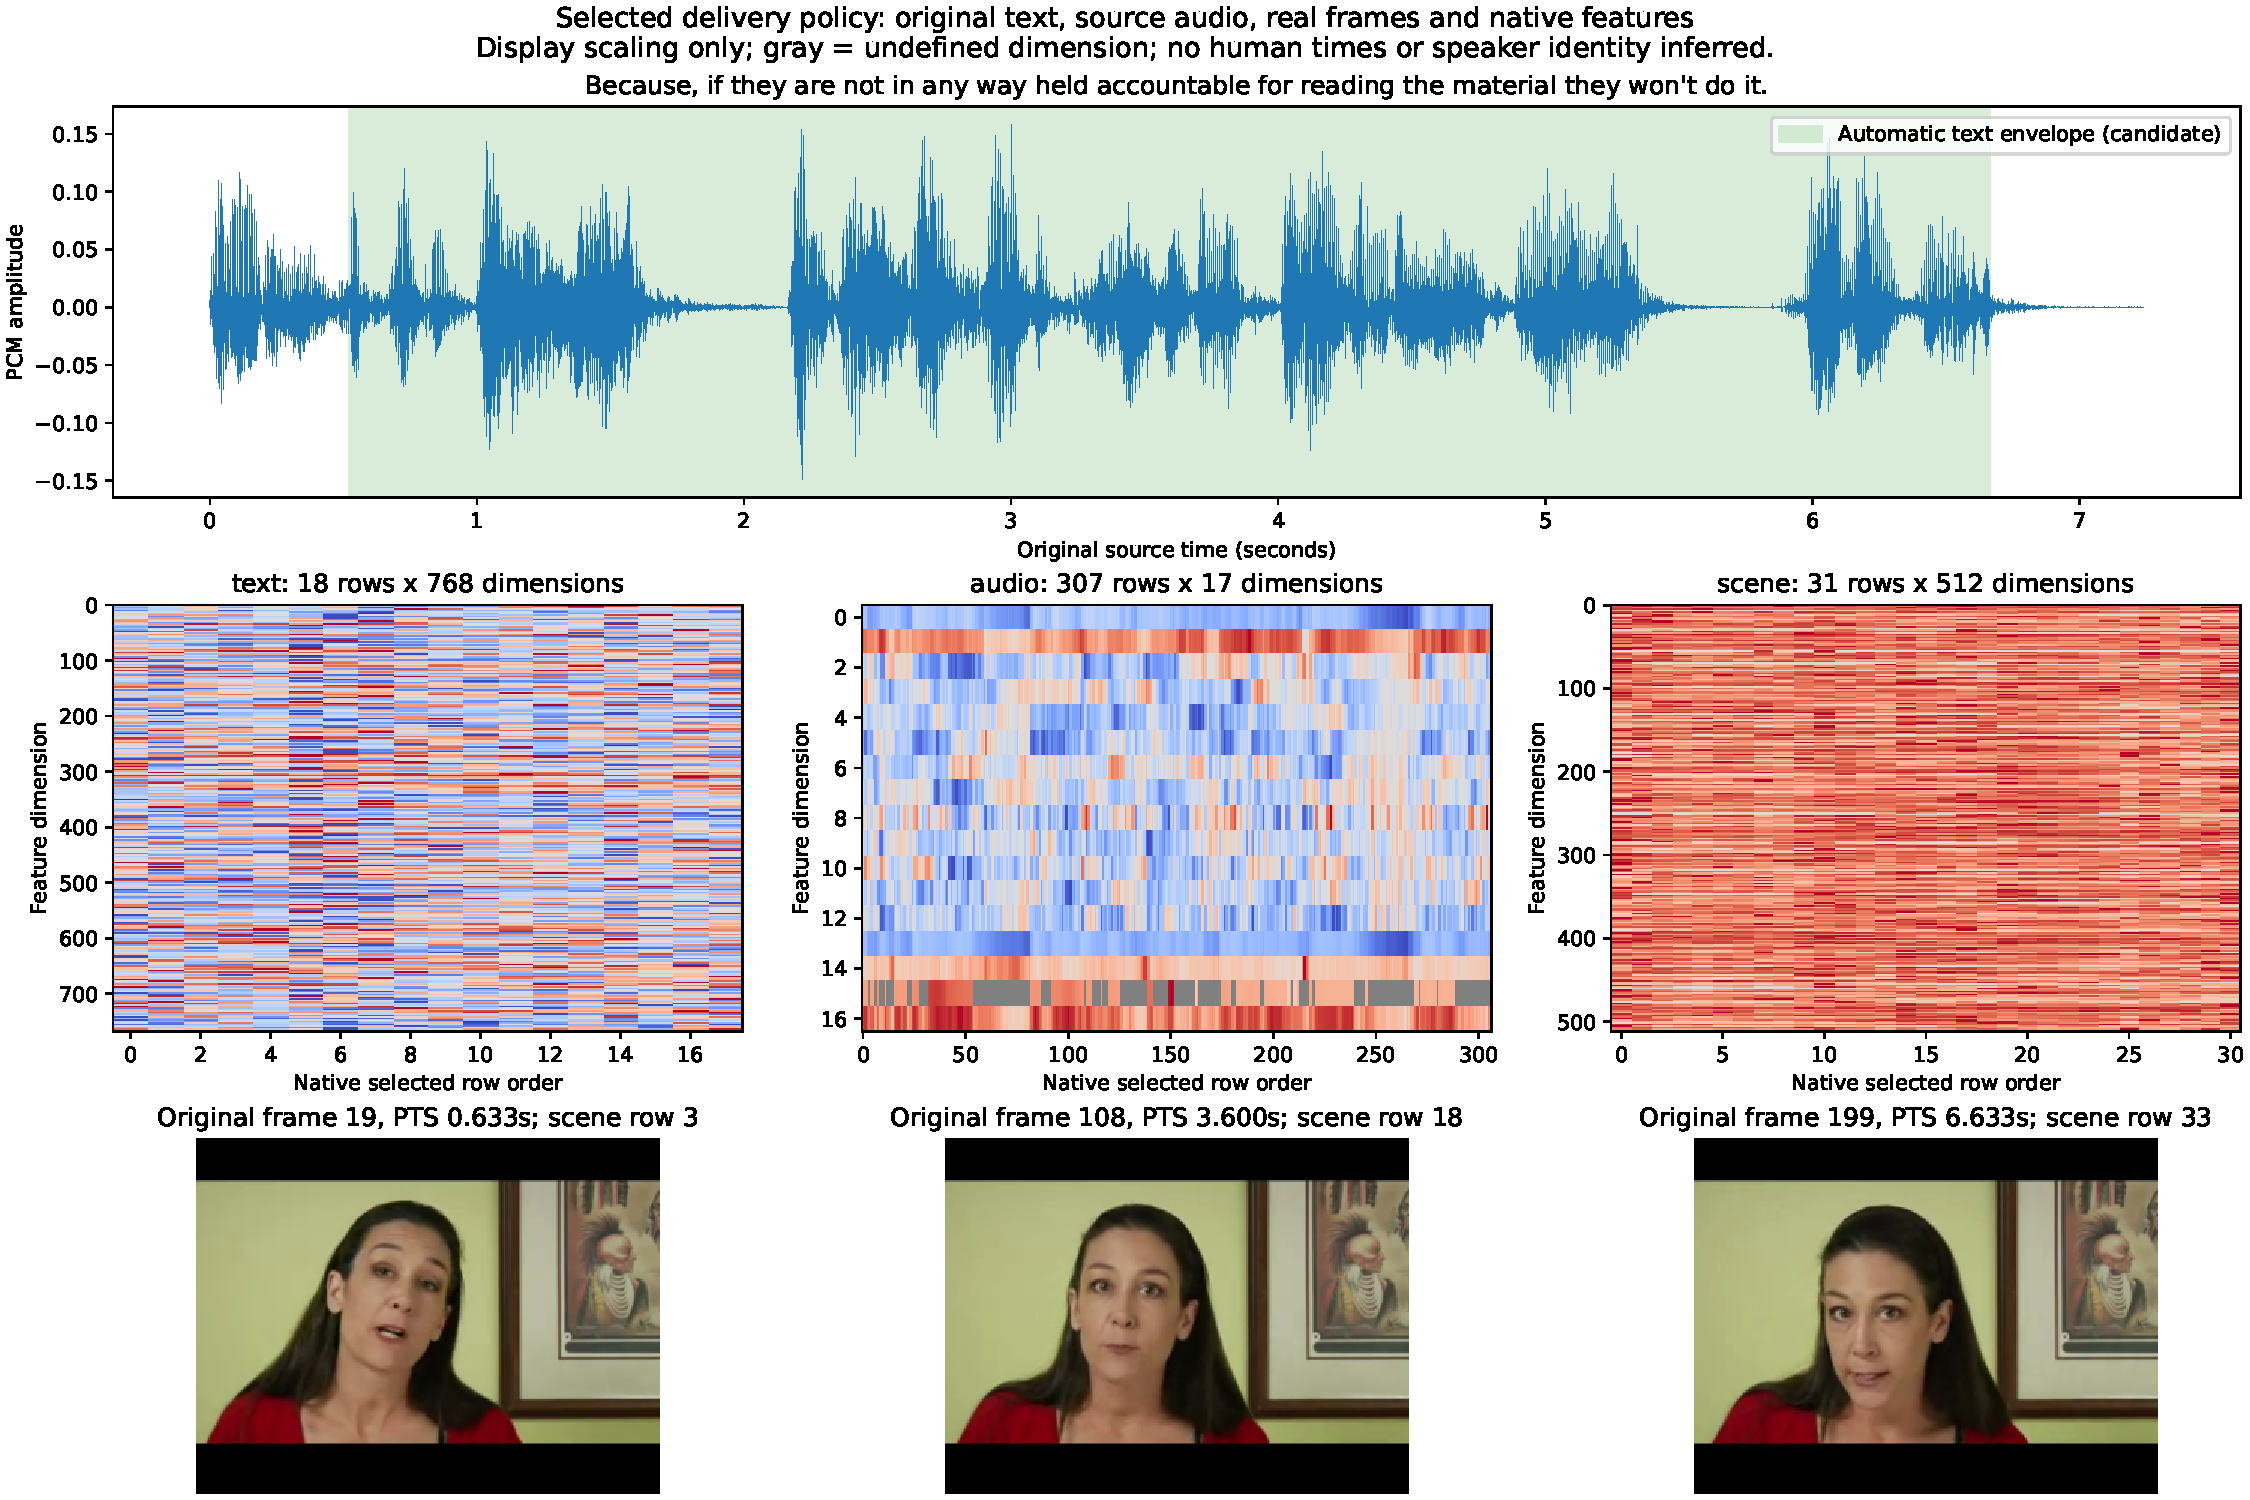
\includegraphics{../问题1/data/figures/delivery_example.pdf}
\caption{自动选择样本的真实三模态实例}
\end{figure}

原帧编号为19、108、199，PTS分别为0.633、3.600、6.633秒。音频区间按候选词界组织，画面按实际时间展示同期场景。物理支持运算排除约4.2088秒源视频空缺；对2759个有有效音高的节点，按逐维有效时长归一化，避免缺失音高填零对聚合值的稀释。

物理支持运算排除了约4.2088秒源视频空缺；2759个有有效音高的节点中，按总时间平均填零音高会压低数值，逐维有效时长归一化避免该稀释。该实验验证物理支持与逐维归一化的实际作用。

\hypertarget{q1-ux53c2ux6570ux914dux7f6eux4e0eux91cdux5efaux6d41ux7a0b}{%
\subsection{参数配置与重建流程}\label{q1-ux53c2ux6570ux914dux7f6eux4e0eux91cdux5efaux6d41ux7a0b}}

\begin{PaperTable}{2}

\begin{longtable}[]{@{}ll@{}}
\caption{参数配置与重建流程}\tabularnewline
\toprule
\begin{minipage}[b]{0.17\columnwidth}\raggedright
环节\strut
\end{minipage} & \begin{minipage}[b]{0.77\columnwidth}\raggedright
工具及固定配置\strut
\end{minipage}\tabularnewline
\midrule
\endfirsthead
\caption[]{参数配置与重建流程（续）}\tabularnewline
\toprule
\begin{minipage}[b]{0.17\columnwidth}\raggedright
环节\strut
\end{minipage} & \begin{minipage}[b]{0.77\columnwidth}\raggedright
工具及固定配置\strut
\end{minipage}\tabularnewline
\midrule
\endhead
\begin{minipage}[t]{0.17\columnwidth}\raggedright
基础环境\strut
\end{minipage} & \begin{minipage}[t]{0.77\columnwidth}\raggedright
Python 3.10；FFmpeg/FFprobe 4.4.2；PyTorch/torchaudio 2.6.0 CPU；torchvision 0.21.0；transformers 4.48.3；MediaPipe 0.10.21\strut
\end{minipage}\tabularnewline
\begin{minipage}[t]{0.17\columnwidth}\raggedright
基础推理\strut
\end{minipage} & \begin{minipage}[t]{0.77\columnwidth}\raggedright
\texttt{distilbe\allowbreak{}rt-\allowbreak{}base-\allowbreak{}uncased}；\texttt{facebook\allowbreak{}/\allowbreak{}wav2vec2\allowbreak{}-\allowbreak{}base-\allowbreak{}960h}；ResNet18 ImageNet1K\_V1；线程2、种子0、推理模式\strut
\end{minipage}\tabularnewline
\begin{minipage}[t]{0.17\columnwidth}\raggedright
独立识别\strut
\end{minipage} & \begin{minipage}[t]{0.77\columnwidth}\raggedright
faster-whisper 1.2.1；CTranslate2 4.8.2；large-v3；RTX 4060、int8\_float16；英语、beam 5、temperature 0、关闭前文条件与VAD\strut
\end{minipage}\tabularnewline
\begin{minipage}[t]{0.17\columnwidth}\raggedright
音素对齐\strut
\end{minipage} & \begin{minipage}[t]{0.77\columnwidth}\raggedright
MFA 3.3.9；english\_mfa v3.0.0声学模型与词典；english\_us\_mfa v3.0.0 G2P；16kHz、beam 10、retry 40、dither 0、关闭说话者适配\strut
\end{minipage}\tabularnewline
\begin{minipage}[t]{0.17\columnwidth}\raggedright
局部边界\strut
\end{minipage} & \begin{minipage}[t]{0.77\columnwidth}\raggedright
上下文扩展0.5秒及1秒；两种上下文与独立识别的端点一致性门槛0.2秒；词组长度2---8词\strut
\end{minipage}\tabularnewline
\bottomrule
\end{longtable}

\end{PaperTable}

运行 \texttt{scripts/\allowbreak{}rebuild\_\allowbreak{}core.py}，传入原始附件目录、固定模型缓存和新输出目录，依次生成素材清单、原生特征、基础关系及物理索引。再由 \texttt{scripts/\allowbreak{}rebuild\_\allowbreak{}multigra\allowbreak{}nular.py} 从原始音轨重做独立识别、裁剪与音素对齐，生成最终词级及词组级关系。模型来源、固定版本与摘要由模型清单记录；NPZ保存数值，JSON保存位置与状态。

同一系统和硬件上，在新安装的Python环境中重建全部100条，1900个原生数组和1200个物理索引数组的类型、形状、数值一致。增强分支在新目录重复生成100条识别输出、236个对齐任务及最终关系，结果一致。该实验验证固定环境、权重和参数下的计算复现。

\hypertarget{q1-ux5168ux90e8100ux6761ux7279ux5f81ux4e0eux65f6ux5e8fux7ed3ux679c}{%
\subsection{全部100条特征与时序结果}\label{q1-ux5168ux90e8100ux6761ux7279ux5f81ux4e0eux65f6ux5e8fux7ed3ux679c}}

T、A、V、F依次表示文本、声音、画面、人脸事件，特征维度分别为768、17、512、52。表中列出各序列长度，乘相应维度即为完整矩阵形状。A/V时长为实际PCM与源帧支持并集的秒数，保留三位小数；文本按词和字符区间定位，人脸按所属帧定位。W/P/U分别为词级候选数、仅词组覆盖词数、完全未确定词数，逐行之和等于T长度。星号标记全零音轨，其物理时长保留而声音使用掩码为false；其他声音轨迹仍采用逐维掩码。

\begin{PaperTable}{5}

\begin{longtable}[]{@{}lrrll@{}}
\caption{全部100条特征与时序结果}\tabularnewline
\toprule
\begin{minipage}[b]{0.29\columnwidth}\raggedright
样本标识\strut
\end{minipage} & \begin{minipage}[b]{0.10\columnwidth}\raggedleft
A秒\strut
\end{minipage} & \begin{minipage}[b]{0.10\columnwidth}\raggedleft
V秒\strut
\end{minipage} & \begin{minipage}[b]{0.24\columnwidth}\raggedright
T/A/V/F长度\strut
\end{minipage} & \begin{minipage}[b]{0.13\columnwidth}\raggedright
W/P/U\strut
\end{minipage}\tabularnewline
\midrule
\endfirsthead
\caption[]{全部100条特征与时序结果（续）}\tabularnewline
\toprule
\begin{minipage}[b]{0.29\columnwidth}\raggedright
样本标识\strut
\end{minipage} & \begin{minipage}[b]{0.10\columnwidth}\raggedleft
A秒\strut
\end{minipage} & \begin{minipage}[b]{0.10\columnwidth}\raggedleft
V秒\strut
\end{minipage} & \begin{minipage}[b]{0.24\columnwidth}\raggedright
T/A/V/F长度\strut
\end{minipage} & \begin{minipage}[b]{0.13\columnwidth}\raggedright
W/P/U\strut
\end{minipage}\tabularnewline
\midrule
\endhead
\begin{minipage}[t]{0.29\columnwidth}\raggedright
\texttt{-\allowbreak{}3g5yACwY\allowbreak{}nA\$\allowbreak{}\_\allowbreak{}\$\allowbreak{}13}\strut
\end{minipage} & \begin{minipage}[t]{0.10\columnwidth}\raggedleft
5.399\strut
\end{minipage} & \begin{minipage}[t]{0.10\columnwidth}\raggedleft
5.433\strut
\end{minipage} & \begin{minipage}[t]{0.24\columnwidth}\raggedright
15/269/29/29\strut
\end{minipage} & \begin{minipage}[t]{0.13\columnwidth}\raggedright
14/1/0\strut
\end{minipage}\tabularnewline
\begin{minipage}[t]{0.29\columnwidth}\raggedright
\texttt{-\allowbreak{}3g5yACwY\allowbreak{}nA\$\allowbreak{}\_\allowbreak{}\$\allowbreak{}2}\strut
\end{minipage} & \begin{minipage}[t]{0.10\columnwidth}\raggedleft
9.231\strut
\end{minipage} & \begin{minipage}[t]{0.10\columnwidth}\raggedleft
9.267\strut
\end{minipage} & \begin{minipage}[t]{0.24\columnwidth}\raggedright
14/461/47/47\strut
\end{minipage} & \begin{minipage}[t]{0.13\columnwidth}\raggedright
12/0/2\strut
\end{minipage}\tabularnewline
\begin{minipage}[t]{0.29\columnwidth}\raggedright
\texttt{-\allowbreak{}3g5yACwY\allowbreak{}nA\$\allowbreak{}\_\allowbreak{}\$\allowbreak{}3}\strut
\end{minipage} & \begin{minipage}[t]{0.10\columnwidth}\raggedleft
14.328\strut
\end{minipage} & \begin{minipage}[t]{0.10\columnwidth}\raggedleft
14.367\strut
\end{minipage} & \begin{minipage}[t]{0.24\columnwidth}\raggedright
29/716/73/73\strut
\end{minipage} & \begin{minipage}[t]{0.13\columnwidth}\raggedright
21/6/2\strut
\end{minipage}\tabularnewline
\begin{minipage}[t]{0.29\columnwidth}\raggedright
\texttt{-\allowbreak{}3g5yACwY\allowbreak{}nA\$\allowbreak{}\_\allowbreak{}\$\allowbreak{}9}\strut
\end{minipage} & \begin{minipage}[t]{0.10\columnwidth}\raggedleft
8.696\strut
\end{minipage} & \begin{minipage}[t]{0.10\columnwidth}\raggedleft
8.767\strut
\end{minipage} & \begin{minipage}[t]{0.24\columnwidth}\raggedright
23/434/45/45\strut
\end{minipage} & \begin{minipage}[t]{0.13\columnwidth}\raggedright
19/3/1\strut
\end{minipage}\tabularnewline
\begin{minipage}[t]{0.29\columnwidth}\raggedright
\texttt{-\allowbreak{}3nNcZdcd\allowbreak{}vU\$\allowbreak{}\_\allowbreak{}\$\allowbreak{}5}\strut
\end{minipage} & \begin{minipage}[t]{0.10\columnwidth}\raggedleft
7.789\strut
\end{minipage} & \begin{minipage}[t]{0.10\columnwidth}\raggedleft
7.867\strut
\end{minipage} & \begin{minipage}[t]{0.24\columnwidth}\raggedright
18/389/40/39\strut
\end{minipage} & \begin{minipage}[t]{0.13\columnwidth}\raggedright
16/0/2\strut
\end{minipage}\tabularnewline
\begin{minipage}[t]{0.29\columnwidth}\raggedright
\texttt{-\allowbreak{}571d8cVa\allowbreak{}uQ\$\allowbreak{}\_\allowbreak{}\$\allowbreak{}0}\strut
\end{minipage} & \begin{minipage}[t]{0.10\columnwidth}\raggedleft
4.992\strut
\end{minipage} & \begin{minipage}[t]{0.10\columnwidth}\raggedleft
5.067\strut
\end{minipage} & \begin{minipage}[t]{0.24\columnwidth}\raggedright
12/249/27/26\strut
\end{minipage} & \begin{minipage}[t]{0.13\columnwidth}\raggedright
7/0/5\strut
\end{minipage}\tabularnewline
\begin{minipage}[t]{0.29\columnwidth}\raggedright
\texttt{-\allowbreak{}571d8cVa\allowbreak{}uQ\$\allowbreak{}\_\allowbreak{}\$\allowbreak{}5}\strut
\end{minipage} & \begin{minipage}[t]{0.10\columnwidth}\raggedleft
15.115\strut
\end{minipage} & \begin{minipage}[t]{0.10\columnwidth}\raggedleft
15.167\strut
\end{minipage} & \begin{minipage}[t]{0.24\columnwidth}\raggedright
43/755/77/77\strut
\end{minipage} & \begin{minipage}[t]{0.13\columnwidth}\raggedright
41/1/1\strut
\end{minipage}\tabularnewline
\begin{minipage}[t]{0.29\columnwidth}\raggedright
\texttt{-\allowbreak{}6rXp3zJ3\allowbreak{}kc\$\allowbreak{}\_\allowbreak{}\$\allowbreak{}8}\strut
\end{minipage} & \begin{minipage}[t]{0.10\columnwidth}\raggedleft
12.738\strut
\end{minipage} & \begin{minipage}[t]{0.10\columnwidth}\raggedleft
12.800\strut
\end{minipage} & \begin{minipage}[t]{0.24\columnwidth}\raggedright
34/636/65/65\strut
\end{minipage} & \begin{minipage}[t]{0.13\columnwidth}\raggedright
30/1/3\strut
\end{minipage}\tabularnewline
\begin{minipage}[t]{0.29\columnwidth}\raggedright
\texttt{-\allowbreak{}9y-\allowbreak{}fZ3swSY\$\allowbreak{}\_\allowbreak{}\$\allowbreak{}0}\strut
\end{minipage} & \begin{minipage}[t]{0.10\columnwidth}\raggedleft
6.757\strut
\end{minipage} & \begin{minipage}[t]{0.10\columnwidth}\raggedleft
6.833\strut
\end{minipage} & \begin{minipage}[t]{0.24\columnwidth}\raggedright
22/337/35/35\strut
\end{minipage} & \begin{minipage}[t]{0.13\columnwidth}\raggedright
11/1/10\strut
\end{minipage}\tabularnewline
\begin{minipage}[t]{0.29\columnwidth}\raggedright
\texttt{-\allowbreak{}9y-\allowbreak{}fZ3swSY\$\allowbreak{}\_\allowbreak{}\$\allowbreak{}4}\strut
\end{minipage} & \begin{minipage}[t]{0.10\columnwidth}\raggedleft
2.665\strut
\end{minipage} & \begin{minipage}[t]{0.10\columnwidth}\raggedleft
2.700\strut
\end{minipage} & \begin{minipage}[t]{0.24\columnwidth}\raggedright
9/132/15/15\strut
\end{minipage} & \begin{minipage}[t]{0.13\columnwidth}\raggedright
4/3/2\strut
\end{minipage}\tabularnewline
\begin{minipage}[t]{0.29\columnwidth}\raggedright
\texttt{-\allowbreak{}9y-\allowbreak{}fZ3swSY\$\allowbreak{}\_\allowbreak{}\$\allowbreak{}8}\strut
\end{minipage} & \begin{minipage}[t]{0.10\columnwidth}\raggedleft
4.917\strut
\end{minipage} & \begin{minipage}[t]{0.10\columnwidth}\raggedleft
4.967\strut
\end{minipage} & \begin{minipage}[t]{0.24\columnwidth}\raggedright
12/245/26/23\strut
\end{minipage} & \begin{minipage}[t]{0.13\columnwidth}\raggedright
12/0/0\strut
\end{minipage}\tabularnewline
\begin{minipage}[t]{0.29\columnwidth}\raggedright
\texttt{-\allowbreak{}AUZQgSxy\allowbreak{}PQ\$\allowbreak{}\_\allowbreak{}\$\allowbreak{}2}\strut
\end{minipage} & \begin{minipage}[t]{0.10\columnwidth}\raggedleft
22.405\strut
\end{minipage} & \begin{minipage}[t]{0.10\columnwidth}\raggedleft
22.467\strut
\end{minipage} & \begin{minipage}[t]{0.24\columnwidth}\raggedright
41/1119/113/113\strut
\end{minipage} & \begin{minipage}[t]{0.13\columnwidth}\raggedright
15/3/23\strut
\end{minipage}\tabularnewline
\begin{minipage}[t]{0.29\columnwidth}\raggedright
\texttt{-\allowbreak{}HeZS2-\allowbreak{}Prhc\$\allowbreak{}\_\allowbreak{}\$\allowbreak{}2}\strut
\end{minipage} & \begin{minipage}[t]{0.10\columnwidth}\raggedleft
8.151\strut
\end{minipage} & \begin{minipage}[t]{0.10\columnwidth}\raggedleft
8.200\strut
\end{minipage} & \begin{minipage}[t]{0.24\columnwidth}\raggedright
16/407/42/42\strut
\end{minipage} & \begin{minipage}[t]{0.13\columnwidth}\raggedright
11/2/3\strut
\end{minipage}\tabularnewline
\begin{minipage}[t]{0.29\columnwidth}\raggedright
\texttt{-\allowbreak{}HwX2H8Z4\allowbreak{}hY\$\allowbreak{}\_\allowbreak{}\$\allowbreak{}2}\strut
\end{minipage} & \begin{minipage}[t]{0.10\columnwidth}\raggedleft
3.916\strut
\end{minipage} & \begin{minipage}[t]{0.10\columnwidth}\raggedleft
3.967\strut
\end{minipage} & \begin{minipage}[t]{0.24\columnwidth}\raggedright
7/195/21/5\strut
\end{minipage} & \begin{minipage}[t]{0.13\columnwidth}\raggedright
0/0/7\strut
\end{minipage}\tabularnewline
\begin{minipage}[t]{0.29\columnwidth}\raggedright
\texttt{-\allowbreak{}HwX2H8Z4\allowbreak{}hY\$\allowbreak{}\_\allowbreak{}\$\allowbreak{}5}\strut
\end{minipage} & \begin{minipage}[t]{0.10\columnwidth}\raggedleft
5.544\strut
\end{minipage} & \begin{minipage}[t]{0.10\columnwidth}\raggedleft
5.600\strut
\end{minipage} & \begin{minipage}[t]{0.24\columnwidth}\raggedright
9/276/29/10\strut
\end{minipage} & \begin{minipage}[t]{0.13\columnwidth}\raggedright
7/0/2\strut
\end{minipage}\tabularnewline
\begin{minipage}[t]{0.29\columnwidth}\raggedright
\texttt{-\allowbreak{}HwX2H8Z4\allowbreak{}hY\$\allowbreak{}\_\allowbreak{}\$\allowbreak{}6}\strut
\end{minipage} & \begin{minipage}[t]{0.10\columnwidth}\raggedleft
3.256\strut
\end{minipage} & \begin{minipage}[t]{0.10\columnwidth}\raggedleft
3.300\strut
\end{minipage} & \begin{minipage}[t]{0.24\columnwidth}\raggedright
7/162/18/11\strut
\end{minipage} & \begin{minipage}[t]{0.13\columnwidth}\raggedright
5/1/1\strut
\end{minipage}\tabularnewline
\begin{minipage}[t]{0.29\columnwidth}\raggedright
\texttt{-\allowbreak{}HwX2H8Z4\allowbreak{}hY\$\allowbreak{}\_\allowbreak{}\$\allowbreak{}9}\strut
\end{minipage} & \begin{minipage}[t]{0.10\columnwidth}\raggedleft
7.636\strut
\end{minipage} & \begin{minipage}[t]{0.10\columnwidth}\raggedleft
7.733\strut
\end{minipage} & \begin{minipage}[t]{0.24\columnwidth}\raggedright
22/381/40/0\strut
\end{minipage} & \begin{minipage}[t]{0.13\columnwidth}\raggedright
6/2/14\strut
\end{minipage}\tabularnewline
\begin{minipage}[t]{0.29\columnwidth}\raggedright
\texttt{-\allowbreak{}I\_\allowbreak{}e4mIh0yE\allowbreak{}\$\allowbreak{}\_\allowbreak{}\$\allowbreak{}1}\strut
\end{minipage} & \begin{minipage}[t]{0.10\columnwidth}\raggedleft
7.444\strut
\end{minipage} & \begin{minipage}[t]{0.10\columnwidth}\raggedleft
7.500\strut
\end{minipage} & \begin{minipage}[t]{0.24\columnwidth}\raggedright
18/371/39/39\strut
\end{minipage} & \begin{minipage}[t]{0.13\columnwidth}\raggedright
18/0/0\strut
\end{minipage}\tabularnewline
\begin{minipage}[t]{0.29\columnwidth}\raggedright
\texttt{-\allowbreak{}I\_\allowbreak{}e4mIh0yE\allowbreak{}\$\allowbreak{}\_\allowbreak{}\$\allowbreak{}3}\strut
\end{minipage} & \begin{minipage}[t]{0.10\columnwidth}\raggedleft
8.994\strut
\end{minipage} & \begin{minipage}[t]{0.10\columnwidth}\raggedleft
9.033\strut
\end{minipage} & \begin{minipage}[t]{0.24\columnwidth}\raggedright
22/449/46/46\strut
\end{minipage} & \begin{minipage}[t]{0.13\columnwidth}\raggedright
17/0/5\strut
\end{minipage}\tabularnewline
\begin{minipage}[t]{0.29\columnwidth}\raggedright
\texttt{-\allowbreak{}MeTTeMJB\allowbreak{}Nc\$\allowbreak{}\_\allowbreak{}\$\allowbreak{}0}\strut
\end{minipage} & \begin{minipage}[t]{0.10\columnwidth}\raggedleft
9.218\strut
\end{minipage} & \begin{minipage}[t]{0.10\columnwidth}\raggedleft
9.300\strut
\end{minipage} & \begin{minipage}[t]{0.24\columnwidth}\raggedright
21/460/48/47\strut
\end{minipage} & \begin{minipage}[t]{0.13\columnwidth}\raggedright
20/0/1\strut
\end{minipage}\tabularnewline
\begin{minipage}[t]{0.29\columnwidth}\raggedright
\texttt{-\allowbreak{}MeTTeMJB\allowbreak{}Nc\$\allowbreak{}\_\allowbreak{}\$\allowbreak{}13}\strut
\end{minipage} & \begin{minipage}[t]{0.10\columnwidth}\raggedleft
5.256\strut
\end{minipage} & \begin{minipage}[t]{0.10\columnwidth}\raggedleft
5.300\strut
\end{minipage} & \begin{minipage}[t]{0.24\columnwidth}\raggedright
14/262/28/28\strut
\end{minipage} & \begin{minipage}[t]{0.13\columnwidth}\raggedright
12/0/2\strut
\end{minipage}\tabularnewline
\begin{minipage}[t]{0.29\columnwidth}\raggedright
\texttt{-\allowbreak{}MeTTeMJB\allowbreak{}Nc\$\allowbreak{}\_\allowbreak{}\$\allowbreak{}7}\strut
\end{minipage} & \begin{minipage}[t]{0.10\columnwidth}\raggedleft
10.411\strut
\end{minipage} & \begin{minipage}[t]{0.10\columnwidth}\raggedleft
10.467\strut
\end{minipage} & \begin{minipage}[t]{0.24\columnwidth}\raggedright
31/520/54/54\strut
\end{minipage} & \begin{minipage}[t]{0.13\columnwidth}\raggedright
31/0/0\strut
\end{minipage}\tabularnewline
\begin{minipage}[t]{0.29\columnwidth}\raggedright
\texttt{-\allowbreak{}NFrJFQij\allowbreak{}FE\$\allowbreak{}\_\allowbreak{}\$\allowbreak{}1}\strut
\end{minipage} & \begin{minipage}[t]{0.10\columnwidth}\raggedleft
5.659\strut
\end{minipage} & \begin{minipage}[t]{0.10\columnwidth}\raggedleft
5.680\strut
\end{minipage} & \begin{minipage}[t]{0.24\columnwidth}\raggedright
16/282/29/0\strut
\end{minipage} & \begin{minipage}[t]{0.13\columnwidth}\raggedright
0/0/16\strut
\end{minipage}\tabularnewline
\begin{minipage}[t]{0.29\columnwidth}\raggedright
\texttt{-\allowbreak{}NFrJFQij\allowbreak{}FE\$\allowbreak{}\_\allowbreak{}\$\allowbreak{}2}\strut
\end{minipage} & \begin{minipage}[t]{0.10\columnwidth}\raggedleft
6.698\strut
\end{minipage} & \begin{minipage}[t]{0.10\columnwidth}\raggedleft
6.760\strut
\end{minipage} & \begin{minipage}[t]{0.24\columnwidth}\raggedright
18/334/35/0\strut
\end{minipage} & \begin{minipage}[t]{0.13\columnwidth}\raggedright
0/0/18\strut
\end{minipage}\tabularnewline
\begin{minipage}[t]{0.29\columnwidth}\raggedright
\texttt{-\allowbreak{}RfYyzHpj\allowbreak{}k4\$\allowbreak{}\_\allowbreak{}\$\allowbreak{}11}\strut
\end{minipage} & \begin{minipage}[t]{0.10\columnwidth}\raggedleft
5.075\strut
\end{minipage} & \begin{minipage}[t]{0.10\columnwidth}\raggedleft
5.133\strut
\end{minipage} & \begin{minipage}[t]{0.24\columnwidth}\raggedright
17/253/27/27\strut
\end{minipage} & \begin{minipage}[t]{0.13\columnwidth}\raggedright
13/3/1\strut
\end{minipage}\tabularnewline
\begin{minipage}[t]{0.29\columnwidth}\raggedright
\texttt{-\allowbreak{}RfYyzHpj\allowbreak{}k4\$\allowbreak{}\_\allowbreak{}\$\allowbreak{}2}\strut
\end{minipage} & \begin{minipage}[t]{0.10\columnwidth}\raggedleft
5.392\strut
\end{minipage} & \begin{minipage}[t]{0.10\columnwidth}\raggedleft
5.467\strut
\end{minipage} & \begin{minipage}[t]{0.24\columnwidth}\raggedright
25/269/29/29\strut
\end{minipage} & \begin{minipage}[t]{0.13\columnwidth}\raggedright
22/3/0\strut
\end{minipage}\tabularnewline
\begin{minipage}[t]{0.29\columnwidth}\raggedright
\texttt{-\allowbreak{}RfYyzHpj\allowbreak{}k4\$\allowbreak{}\_\allowbreak{}\$\allowbreak{}8}\strut
\end{minipage} & \begin{minipage}[t]{0.10\columnwidth}\raggedleft
4.532\strut
\end{minipage} & \begin{minipage}[t]{0.10\columnwidth}\raggedleft
4.567\strut
\end{minipage} & \begin{minipage}[t]{0.24\columnwidth}\raggedright
17/226/24/24\strut
\end{minipage} & \begin{minipage}[t]{0.13\columnwidth}\raggedright
16/0/1\strut
\end{minipage}\tabularnewline
\begin{minipage}[t]{0.29\columnwidth}\raggedright
\texttt{-\allowbreak{}THoVjtIk\allowbreak{}eU\$\allowbreak{}\_\allowbreak{}\$\allowbreak{}12}\strut
\end{minipage} & \begin{minipage}[t]{0.10\columnwidth}\raggedleft
14.806\strut
\end{minipage} & \begin{minipage}[t]{0.10\columnwidth}\raggedleft
14.833\strut
\end{minipage} & \begin{minipage}[t]{0.24\columnwidth}\raggedright
39/740/75/75\strut
\end{minipage} & \begin{minipage}[t]{0.13\columnwidth}\raggedright
35/0/4\strut
\end{minipage}\tabularnewline
\begin{minipage}[t]{0.29\columnwidth}\raggedright
\texttt{-\allowbreak{}THoVjtIk\allowbreak{}eU\$\allowbreak{}\_\allowbreak{}\$\allowbreak{}2}\strut
\end{minipage} & \begin{minipage}[t]{0.10\columnwidth}\raggedleft
4.231\strut
\end{minipage} & \begin{minipage}[t]{0.10\columnwidth}\raggedleft
4.267\strut
\end{minipage} & \begin{minipage}[t]{0.24\columnwidth}\raggedright
10/211/23/23\strut
\end{minipage} & \begin{minipage}[t]{0.13\columnwidth}\raggedright
10/0/0\strut
\end{minipage}\tabularnewline
\begin{minipage}[t]{0.29\columnwidth}\raggedright
\texttt{-\allowbreak{}THoVjtIk\allowbreak{}eU\$\allowbreak{}\_\allowbreak{}\$\allowbreak{}6}\strut
\end{minipage} & \begin{minipage}[t]{0.10\columnwidth}\raggedleft
7.983\strut
\end{minipage} & \begin{minipage}[t]{0.10\columnwidth}\raggedleft
8.033\strut
\end{minipage} & \begin{minipage}[t]{0.24\columnwidth}\raggedright
30/398/41/41\strut
\end{minipage} & \begin{minipage}[t]{0.13\columnwidth}\raggedright
27/0/3\strut
\end{minipage}\tabularnewline
\begin{minipage}[t]{0.29\columnwidth}\raggedright
\texttt{-\allowbreak{}UUCSKoHe\allowbreak{}MA\$\allowbreak{}\_\allowbreak{}\$\allowbreak{}0}\strut
\end{minipage} & \begin{minipage}[t]{0.10\columnwidth}\raggedleft
7.732\strut
\end{minipage} & \begin{minipage}[t]{0.10\columnwidth}\raggedleft
7.800\strut
\end{minipage} & \begin{minipage}[t]{0.24\columnwidth}\raggedright
18/386/40/39\strut
\end{minipage} & \begin{minipage}[t]{0.13\columnwidth}\raggedright
16/2/0\strut
\end{minipage}\tabularnewline
\begin{minipage}[t]{0.29\columnwidth}\raggedright
\texttt{-\allowbreak{}UacrmKiT\allowbreak{}n4\$\allowbreak{}\_\allowbreak{}\$\allowbreak{}10}\strut
\end{minipage} & \begin{minipage}[t]{0.10\columnwidth}\raggedleft
7.242\strut
\end{minipage} & \begin{minipage}[t]{0.10\columnwidth}\raggedleft
7.267\strut
\end{minipage} & \begin{minipage}[t]{0.24\columnwidth}\raggedright
18/361/38/38\strut
\end{minipage} & \begin{minipage}[t]{0.13\columnwidth}\raggedright
18/0/0\strut
\end{minipage}\tabularnewline
\begin{minipage}[t]{0.29\columnwidth}\raggedright
\texttt{-\allowbreak{}UacrmKiT\allowbreak{}n4\$\allowbreak{}\_\allowbreak{}\$\allowbreak{}4}\strut
\end{minipage} & \begin{minipage}[t]{0.10\columnwidth}\raggedleft
4.682\strut
\end{minipage} & \begin{minipage}[t]{0.10\columnwidth}\raggedleft
4.733\strut
\end{minipage} & \begin{minipage}[t]{0.24\columnwidth}\raggedright
14/233/25/25\strut
\end{minipage} & \begin{minipage}[t]{0.13\columnwidth}\raggedright
13/0/1\strut
\end{minipage}\tabularnewline
\begin{minipage}[t]{0.29\columnwidth}\raggedright
\texttt{-\allowbreak{}UuX1xuai\allowbreak{}iE\$\allowbreak{}\_\allowbreak{}\$\allowbreak{}0}\strut
\end{minipage} & \begin{minipage}[t]{0.10\columnwidth}\raggedleft
3.576\strut
\end{minipage} & \begin{minipage}[t]{0.10\columnwidth}\raggedleft
3.633\strut
\end{minipage} & \begin{minipage}[t]{0.24\columnwidth}\raggedright
9/178/20/29\strut
\end{minipage} & \begin{minipage}[t]{0.13\columnwidth}\raggedright
8/1/0\strut
\end{minipage}\tabularnewline
\begin{minipage}[t]{0.29\columnwidth}\raggedright
\texttt{-\allowbreak{}UuX1xuai\allowbreak{}iE\$\allowbreak{}\_\allowbreak{}\$\allowbreak{}1}\strut
\end{minipage} & \begin{minipage}[t]{0.10\columnwidth}\raggedleft
10.267\strut
\end{minipage} & \begin{minipage}[t]{0.10\columnwidth}\raggedleft
10.300\strut
\end{minipage} & \begin{minipage}[t]{0.24\columnwidth}\raggedright
27/513/53/105\strut
\end{minipage} & \begin{minipage}[t]{0.13\columnwidth}\raggedright
24/2/1\strut
\end{minipage}\tabularnewline
\begin{minipage}[t]{0.29\columnwidth}\raggedright
\texttt{-\allowbreak{}UuX1xuai\allowbreak{}iE\$\allowbreak{}\_\allowbreak{}\$\allowbreak{}3}\strut
\end{minipage} & \begin{minipage}[t]{0.10\columnwidth}\raggedleft
4.038\strut
\end{minipage} & \begin{minipage}[t]{0.10\columnwidth}\raggedleft
4.100\strut
\end{minipage} & \begin{minipage}[t]{0.24\columnwidth}\raggedright
9/201/22/22\strut
\end{minipage} & \begin{minipage}[t]{0.13\columnwidth}\raggedright
7/1/1\strut
\end{minipage}\tabularnewline
\begin{minipage}[t]{0.29\columnwidth}\raggedright
\texttt{-\allowbreak{}UuX1xuai\allowbreak{}iE\$\allowbreak{}\_\allowbreak{}\$\allowbreak{}6}\strut
\end{minipage} & \begin{minipage}[t]{0.10\columnwidth}\raggedleft
7.944\strut
\end{minipage} & \begin{minipage}[t]{0.10\columnwidth}\raggedleft
8.000\strut
\end{minipage} & \begin{minipage}[t]{0.24\columnwidth}\raggedright
22/396/41/41\strut
\end{minipage} & \begin{minipage}[t]{0.13\columnwidth}\raggedright
17/2/3\strut
\end{minipage}\tabularnewline
\begin{minipage}[t]{0.29\columnwidth}\raggedright
\texttt{-\allowbreak{}a55Q6RWv\allowbreak{}TA\$\allowbreak{}\_\allowbreak{}\$\allowbreak{}3}\strut
\end{minipage} & \begin{minipage}[t]{0.10\columnwidth}\raggedleft
22.083\strut
\end{minipage} & \begin{minipage}[t]{0.10\columnwidth}\raggedleft
22.133\strut
\end{minipage} & \begin{minipage}[t]{0.24\columnwidth}\raggedright
65/1103/112/116\strut
\end{minipage} & \begin{minipage}[t]{0.13\columnwidth}\raggedright
61/2/2\strut
\end{minipage}\tabularnewline
\begin{minipage}[t]{0.29\columnwidth}\raggedright
\texttt{-\allowbreak{}aNfi7CP8\allowbreak{}vM\$\allowbreak{}\_\allowbreak{}\$\allowbreak{}7}\strut
\end{minipage} & \begin{minipage}[t]{0.10\columnwidth}\raggedleft
8.538\strut
\end{minipage} & \begin{minipage}[t]{0.10\columnwidth}\raggedleft
8.567\strut
\end{minipage} & \begin{minipage}[t]{0.24\columnwidth}\raggedright
18/426/44/44\strut
\end{minipage} & \begin{minipage}[t]{0.13\columnwidth}\raggedright
12/2/4\strut
\end{minipage}\tabularnewline
\begin{minipage}[t]{0.29\columnwidth}\raggedright
\texttt{-\allowbreak{}aqamKhZ1\allowbreak{}Ec\$\allowbreak{}\_\allowbreak{}\$\allowbreak{}0}\strut
\end{minipage} & \begin{minipage}[t]{0.10\columnwidth}\raggedleft
10.890\strut
\end{minipage} & \begin{minipage}[t]{0.10\columnwidth}\raggedleft
10.967\strut
\end{minipage} & \begin{minipage}[t]{0.24\columnwidth}\raggedright
14/544/56/56\strut
\end{minipage} & \begin{minipage}[t]{0.13\columnwidth}\raggedright
6/5/3\strut
\end{minipage}\tabularnewline
\begin{minipage}[t]{0.29\columnwidth}\raggedright
\texttt{-\allowbreak{}dxfTGcXJ\allowbreak{}oc\$\allowbreak{}\_\allowbreak{}\$\allowbreak{}0}\strut
\end{minipage} & \begin{minipage}[t]{0.10\columnwidth}\raggedleft
20.410\strut
\end{minipage} & \begin{minipage}[t]{0.10\columnwidth}\raggedleft
20.500\strut
\end{minipage} & \begin{minipage}[t]{0.24\columnwidth}\raggedright
40/1020/104/81\strut
\end{minipage} & \begin{minipage}[t]{0.13\columnwidth}\raggedright
30/1/9\strut
\end{minipage}\tabularnewline
\begin{minipage}[t]{0.29\columnwidth}\raggedright
\texttt{-\allowbreak{}dxfTGcXJ\allowbreak{}oc\$\allowbreak{}\_\allowbreak{}\$\allowbreak{}1}\strut
\end{minipage} & \begin{minipage}[t]{0.10\columnwidth}\raggedleft
16.018\strut
\end{minipage} & \begin{minipage}[t]{0.10\columnwidth}\raggedleft
16.067\strut
\end{minipage} & \begin{minipage}[t]{0.24\columnwidth}\raggedright
37/800/82/82\strut
\end{minipage} & \begin{minipage}[t]{0.13\columnwidth}\raggedright
32/4/1\strut
\end{minipage}\tabularnewline
\begin{minipage}[t]{0.29\columnwidth}\raggedright
\texttt{-\allowbreak{}dxfTGcXJ\allowbreak{}oc\$\allowbreak{}\_\allowbreak{}\$\allowbreak{}2}\strut
\end{minipage} & \begin{minipage}[t]{0.10\columnwidth}\raggedleft
16.633\strut
\end{minipage} & \begin{minipage}[t]{0.10\columnwidth}\raggedleft
16.667\strut
\end{minipage} & \begin{minipage}[t]{0.24\columnwidth}\raggedright
34/831/85/85\strut
\end{minipage} & \begin{minipage}[t]{0.13\columnwidth}\raggedright
32/0/2\strut
\end{minipage}\tabularnewline
\begin{minipage}[t]{0.29\columnwidth}\raggedright
\texttt{-\allowbreak{}dxfTGcXJ\allowbreak{}oc\$\allowbreak{}\_\allowbreak{}\$\allowbreak{}6}\strut
\end{minipage} & \begin{minipage}[t]{0.10\columnwidth}\raggedleft
12.628\strut
\end{minipage} & \begin{minipage}[t]{0.10\columnwidth}\raggedleft
12.700\strut
\end{minipage} & \begin{minipage}[t]{0.24\columnwidth}\raggedright
28/631/65/65\strut
\end{minipage} & \begin{minipage}[t]{0.13\columnwidth}\raggedright
26/1/1\strut
\end{minipage}\tabularnewline
\begin{minipage}[t]{0.29\columnwidth}\raggedright
\texttt{-\allowbreak{}egA8-\allowbreak{}b7-\allowbreak{}3M\$\allowbreak{}\_\allowbreak{}\$\allowbreak{}1}\strut
\end{minipage} & \begin{minipage}[t]{0.10\columnwidth}\raggedleft
10.156\strut
\end{minipage} & \begin{minipage}[t]{0.10\columnwidth}\raggedleft
10.200\strut
\end{minipage} & \begin{minipage}[t]{0.24\columnwidth}\raggedright
20/507/52/52\strut
\end{minipage} & \begin{minipage}[t]{0.13\columnwidth}\raggedright
15/4/1\strut
\end{minipage}\tabularnewline
\begin{minipage}[t]{0.29\columnwidth}\raggedright
\texttt{-\allowbreak{}egA8-\allowbreak{}b7-\allowbreak{}3M\$\allowbreak{}\_\allowbreak{}\$\allowbreak{}13}\strut
\end{minipage} & \begin{minipage}[t]{0.10\columnwidth}\raggedleft
4.024\strut
\end{minipage} & \begin{minipage}[t]{0.10\columnwidth}\raggedleft
4.100\strut
\end{minipage} & \begin{minipage}[t]{0.24\columnwidth}\raggedright
11/200/22/22\strut
\end{minipage} & \begin{minipage}[t]{0.13\columnwidth}\raggedright
11/0/0\strut
\end{minipage}\tabularnewline
\begin{minipage}[t]{0.29\columnwidth}\raggedright
\texttt{-\allowbreak{}egA8-\allowbreak{}b7-\allowbreak{}3M\$\allowbreak{}\_\allowbreak{}\$\allowbreak{}16}\strut
\end{minipage} & \begin{minipage}[t]{0.10\columnwidth}\raggedleft
5.483\strut
\end{minipage} & \begin{minipage}[t]{0.10\columnwidth}\raggedleft
5.533\strut
\end{minipage} & \begin{minipage}[t]{0.24\columnwidth}\raggedright
11/273/29/29\strut
\end{minipage} & \begin{minipage}[t]{0.13\columnwidth}\raggedright
11/0/0\strut
\end{minipage}\tabularnewline
\begin{minipage}[t]{0.29\columnwidth}\raggedright
\texttt{-\allowbreak{}egA8-\allowbreak{}b7-\allowbreak{}3M\$\allowbreak{}\_\allowbreak{}\$\allowbreak{}17}\strut
\end{minipage} & \begin{minipage}[t]{0.10\columnwidth}\raggedleft
7.095\strut
\end{minipage} & \begin{minipage}[t]{0.10\columnwidth}\raggedleft
7.167\strut
\end{minipage} & \begin{minipage}[t]{0.24\columnwidth}\raggedright
16/354/37/37\strut
\end{minipage} & \begin{minipage}[t]{0.13\columnwidth}\raggedright
15/1/0\strut
\end{minipage}\tabularnewline
\begin{minipage}[t]{0.29\columnwidth}\raggedright
\texttt{-\allowbreak{}egA8-\allowbreak{}b7-\allowbreak{}3M\$\allowbreak{}\_\allowbreak{}\$\allowbreak{}18}\strut
\end{minipage} & \begin{minipage}[t]{0.10\columnwidth}\raggedleft
8.266\strut
\end{minipage} & \begin{minipage}[t]{0.10\columnwidth}\raggedleft
8.333\strut
\end{minipage} & \begin{minipage}[t]{0.24\columnwidth}\raggedright
22/413/43/43\strut
\end{minipage} & \begin{minipage}[t]{0.13\columnwidth}\raggedright
21/1/0\strut
\end{minipage}\tabularnewline
\begin{minipage}[t]{0.29\columnwidth}\raggedright
\texttt{-\allowbreak{}egA8-\allowbreak{}b7-\allowbreak{}3M\$\allowbreak{}\_\allowbreak{}\$\allowbreak{}20}\strut
\end{minipage} & \begin{minipage}[t]{0.10\columnwidth}\raggedleft
6.474\strut
\end{minipage} & \begin{minipage}[t]{0.10\columnwidth}\raggedleft
6.533\strut
\end{minipage} & \begin{minipage}[t]{0.24\columnwidth}\raggedright
20/323/34/34\strut
\end{minipage} & \begin{minipage}[t]{0.13\columnwidth}\raggedright
20/0/0\strut
\end{minipage}\tabularnewline
\begin{minipage}[t]{0.29\columnwidth}\raggedright
\texttt{-\allowbreak{}egA8-\allowbreak{}b7-\allowbreak{}3M\$\allowbreak{}\_\allowbreak{}\$\allowbreak{}26}\strut
\end{minipage} & \begin{minipage}[t]{0.10\columnwidth}\raggedleft
5.921\strut
\end{minipage} & \begin{minipage}[t]{0.10\columnwidth}\raggedleft
5.967\strut
\end{minipage} & \begin{minipage}[t]{0.24\columnwidth}\raggedright
15/295/31/31\strut
\end{minipage} & \begin{minipage}[t]{0.13\columnwidth}\raggedright
14/0/1\strut
\end{minipage}\tabularnewline
\begin{minipage}[t]{0.29\columnwidth}\raggedright
\texttt{-\allowbreak{}egA8-\allowbreak{}b7-\allowbreak{}3M\$\allowbreak{}\_\allowbreak{}\$\allowbreak{}6}\strut
\end{minipage} & \begin{minipage}[t]{0.10\columnwidth}\raggedleft
6.183\strut
\end{minipage} & \begin{minipage}[t]{0.10\columnwidth}\raggedleft
6.233\strut
\end{minipage} & \begin{minipage}[t]{0.24\columnwidth}\raggedright
12/308/32/32\strut
\end{minipage} & \begin{minipage}[t]{0.13\columnwidth}\raggedright
11/0/1\strut
\end{minipage}\tabularnewline
\begin{minipage}[t]{0.29\columnwidth}\raggedright
\texttt{-\allowbreak{}egA8-\allowbreak{}b7-\allowbreak{}3M\$\allowbreak{}\_\allowbreak{}\$\allowbreak{}9}\strut
\end{minipage} & \begin{minipage}[t]{0.10\columnwidth}\raggedleft
4.936\strut
\end{minipage} & \begin{minipage}[t]{0.10\columnwidth}\raggedleft
5.000\strut
\end{minipage} & \begin{minipage}[t]{0.24\columnwidth}\raggedright
10/246/26/26\strut
\end{minipage} & \begin{minipage}[t]{0.13\columnwidth}\raggedright
10/0/0\strut
\end{minipage}\tabularnewline
\begin{minipage}[t]{0.29\columnwidth}\raggedright
\texttt{-\allowbreak{}hnBHBN8p\allowbreak{}5A\$\allowbreak{}\_\allowbreak{}\$\allowbreak{}6}\strut
\end{minipage} & \begin{minipage}[t]{0.10\columnwidth}\raggedleft
6.333\strut
\end{minipage} & \begin{minipage}[t]{0.10\columnwidth}\raggedleft
6.380\strut
\end{minipage} & \begin{minipage}[t]{0.24\columnwidth}\raggedright
13/316/33/17\strut
\end{minipage} & \begin{minipage}[t]{0.13\columnwidth}\raggedright
0/0/13\strut
\end{minipage}\tabularnewline
\begin{minipage}[t]{0.29\columnwidth}\raggedright
\texttt{-\allowbreak{}hnBHBN8p\allowbreak{}5A\$\allowbreak{}\_\allowbreak{}\$\allowbreak{}7}\strut
\end{minipage} & \begin{minipage}[t]{0.10\columnwidth}\raggedleft
7.309\strut
\end{minipage} & \begin{minipage}[t]{0.10\columnwidth}\raggedleft
7.339\strut
\end{minipage} & \begin{minipage}[t]{0.24\columnwidth}\raggedright
13/365/38/29\strut
\end{minipage} & \begin{minipage}[t]{0.13\columnwidth}\raggedright
0/0/13\strut
\end{minipage}\tabularnewline
\begin{minipage}[t]{0.29\columnwidth}\raggedright
\texttt{-\allowbreak{}iRBcNs9o\allowbreak{}I8\$\allowbreak{}\_\allowbreak{}\$\allowbreak{}3}\strut
\end{minipage} & \begin{minipage}[t]{0.10\columnwidth}\raggedleft
5.538\strut
\end{minipage} & \begin{minipage}[t]{0.10\columnwidth}\raggedleft
5.572\strut
\end{minipage} & \begin{minipage}[t]{0.24\columnwidth}\raggedright
8/276/29/29\strut
\end{minipage} & \begin{minipage}[t]{0.13\columnwidth}\raggedright
0/0/8\strut
\end{minipage}\tabularnewline
\begin{minipage}[t]{0.29\columnwidth}\raggedright
\texttt{-\allowbreak{}iRBcNs9o\allowbreak{}I8\$\allowbreak{}\_\allowbreak{}\$\allowbreak{}6}\strut
\end{minipage} & \begin{minipage}[t]{0.10\columnwidth}\raggedleft
2.820\strut
\end{minipage} & \begin{minipage}[t]{0.10\columnwidth}\raggedleft
2.836\strut
\end{minipage} & \begin{minipage}[t]{0.24\columnwidth}\raggedright
5/140/15/15\strut
\end{minipage} & \begin{minipage}[t]{0.13\columnwidth}\raggedright
0/0/5\strut
\end{minipage}\tabularnewline
\begin{minipage}[t]{0.29\columnwidth}\raggedright
\texttt{-\allowbreak{}iRBcNs9o\allowbreak{}I8\$\allowbreak{}\_\allowbreak{}\$\allowbreak{}7}\strut
\end{minipage} & \begin{minipage}[t]{0.10\columnwidth}\raggedleft
4.006\strut
\end{minipage} & \begin{minipage}[t]{0.10\columnwidth}\raggedleft
4.004\strut
\end{minipage} & \begin{minipage}[t]{0.24\columnwidth}\raggedright
9/200/21/21\strut
\end{minipage} & \begin{minipage}[t]{0.13\columnwidth}\raggedright
0/0/9\strut
\end{minipage}\tabularnewline
\begin{minipage}[t]{0.29\columnwidth}\raggedright
\texttt{-\allowbreak{}iRBcNs9o\allowbreak{}I8\$\allowbreak{}\_\allowbreak{}\$\allowbreak{}8}\strut
\end{minipage} & \begin{minipage}[t]{0.10\columnwidth}\raggedleft
8.026\strut
\end{minipage} & \begin{minipage}[t]{0.10\columnwidth}\raggedleft
8.041\strut
\end{minipage} & \begin{minipage}[t]{0.24\columnwidth}\raggedright
21/401/41/41\strut
\end{minipage} & \begin{minipage}[t]{0.13\columnwidth}\raggedright
0/0/21\strut
\end{minipage}\tabularnewline
\begin{minipage}[t]{0.29\columnwidth}\raggedright
\texttt{-\allowbreak{}iRBcNs9o\allowbreak{}I8\$\allowbreak{}\_\allowbreak{}\$\allowbreak{}9}\strut
\end{minipage} & \begin{minipage}[t]{0.10\columnwidth}\raggedleft
3.374\strut
\end{minipage} & \begin{minipage}[t]{0.10\columnwidth}\raggedleft
3.403\strut
\end{minipage} & \begin{minipage}[t]{0.24\columnwidth}\raggedright
5/168/18/13\strut
\end{minipage} & \begin{minipage}[t]{0.13\columnwidth}\raggedright
0/0/5\strut
\end{minipage}\tabularnewline
\begin{minipage}[t]{0.29\columnwidth}\raggedright
\texttt{-\allowbreak{}lzEya4AM\allowbreak{}\_\allowbreak{}4\$\allowbreak{}\_\allowbreak{}\$\allowbreak{}5}\strut
\end{minipage} & \begin{minipage}[t]{0.10\columnwidth}\raggedleft
7.570\strut
\end{minipage} & \begin{minipage}[t]{0.10\columnwidth}\raggedleft
7.633\strut
\end{minipage} & \begin{minipage}[t]{0.24\columnwidth}\raggedright
19/378/39/39\strut
\end{minipage} & \begin{minipage}[t]{0.13\columnwidth}\raggedright
16/1/2\strut
\end{minipage}\tabularnewline
\begin{minipage}[t]{0.29\columnwidth}\raggedright
\texttt{-\allowbreak{}lzEya4AM\allowbreak{}\_\allowbreak{}4\$\allowbreak{}\_\allowbreak{}\$\allowbreak{}6}\strut
\end{minipage} & \begin{minipage}[t]{0.10\columnwidth}\raggedleft
14.740\strut
\end{minipage} & \begin{minipage}[t]{0.10\columnwidth}\raggedleft
14.767\strut
\end{minipage} & \begin{minipage}[t]{0.24\columnwidth}\raggedright
43/736/75/75\strut
\end{minipage} & \begin{minipage}[t]{0.13\columnwidth}\raggedright
39/2/2\strut
\end{minipage}\tabularnewline
\begin{minipage}[t]{0.29\columnwidth}\raggedright
\texttt{-\allowbreak{}mJ2ud6oK\allowbreak{}I8\$\allowbreak{}\_\allowbreak{}\$\allowbreak{}1}*\strut
\end{minipage} & \begin{minipage}[t]{0.10\columnwidth}\raggedleft
6.055\strut
\end{minipage} & \begin{minipage}[t]{0.10\columnwidth}\raggedleft
6.073\strut
\end{minipage} & \begin{minipage}[t]{0.24\columnwidth}\raggedright
13/302/32/0\strut
\end{minipage} & \begin{minipage}[t]{0.13\columnwidth}\raggedright
0/0/13\strut
\end{minipage}\tabularnewline
\begin{minipage}[t]{0.29\columnwidth}\raggedright
\texttt{-\allowbreak{}mJ2ud6oK\allowbreak{}I8\$\allowbreak{}\_\allowbreak{}\$\allowbreak{}2}*\strut
\end{minipage} & \begin{minipage}[t]{0.10\columnwidth}\raggedleft
5.702\strut
\end{minipage} & \begin{minipage}[t]{0.10\columnwidth}\raggedleft
5.706\strut
\end{minipage} & \begin{minipage}[t]{0.24\columnwidth}\raggedright
11/284/30/0\strut
\end{minipage} & \begin{minipage}[t]{0.13\columnwidth}\raggedright
0/0/11\strut
\end{minipage}\tabularnewline
\begin{minipage}[t]{0.29\columnwidth}\raggedright
\texttt{-\allowbreak{}mJ2ud6oK\allowbreak{}I8\$\allowbreak{}\_\allowbreak{}\$\allowbreak{}6}\strut
\end{minipage} & \begin{minipage}[t]{0.10\columnwidth}\raggedleft
2.228\strut
\end{minipage} & \begin{minipage}[t]{0.10\columnwidth}\raggedleft
2.236\strut
\end{minipage} & \begin{minipage}[t]{0.24\columnwidth}\raggedright
5/111/12/12\strut
\end{minipage} & \begin{minipage}[t]{0.13\columnwidth}\raggedright
0/0/5\strut
\end{minipage}\tabularnewline
\begin{minipage}[t]{0.29\columnwidth}\raggedright
\texttt{-\allowbreak{}mJ2ud6oK\allowbreak{}I8\$\allowbreak{}\_\allowbreak{}\$\allowbreak{}8}\strut
\end{minipage} & \begin{minipage}[t]{0.10\columnwidth}\raggedleft
4.171\strut
\end{minipage} & \begin{minipage}[t]{0.10\columnwidth}\raggedleft
4.171\strut
\end{minipage} & \begin{minipage}[t]{0.24\columnwidth}\raggedright
11/208/22/22\strut
\end{minipage} & \begin{minipage}[t]{0.13\columnwidth}\raggedright
0/0/11\strut
\end{minipage}\tabularnewline
\begin{minipage}[t]{0.29\columnwidth}\raggedright
\texttt{-\allowbreak{}mJ2ud6oK\allowbreak{}I8\$\allowbreak{}\_\allowbreak{}\$\allowbreak{}9}\strut
\end{minipage} & \begin{minipage}[t]{0.10\columnwidth}\raggedleft
6.909\strut
\end{minipage} & \begin{minipage}[t]{0.10\columnwidth}\raggedleft
6.940\strut
\end{minipage} & \begin{minipage}[t]{0.24\columnwidth}\raggedright
22/345/36/36\strut
\end{minipage} & \begin{minipage}[t]{0.13\columnwidth}\raggedright
0/0/22\strut
\end{minipage}\tabularnewline
\begin{minipage}[t]{0.29\columnwidth}\raggedright
\texttt{-\allowbreak{}mqbVkbCn\allowbreak{}dg\$\allowbreak{}\_\allowbreak{}\$\allowbreak{}0}\strut
\end{minipage} & \begin{minipage}[t]{0.10\columnwidth}\raggedleft
6.385\strut
\end{minipage} & \begin{minipage}[t]{0.10\columnwidth}\raggedleft
6.467\strut
\end{minipage} & \begin{minipage}[t]{0.24\columnwidth}\raggedright
14/319/34/34\strut
\end{minipage} & \begin{minipage}[t]{0.13\columnwidth}\raggedright
14/0/0\strut
\end{minipage}\tabularnewline
\begin{minipage}[t]{0.29\columnwidth}\raggedright
\texttt{-\allowbreak{}qDkUB0Gg\allowbreak{}YY\$\allowbreak{}\_\allowbreak{}\$\allowbreak{}6}\strut
\end{minipage} & \begin{minipage}[t]{0.10\columnwidth}\raggedleft
4.615\strut
\end{minipage} & \begin{minipage}[t]{0.10\columnwidth}\raggedleft
4.667\strut
\end{minipage} & \begin{minipage}[t]{0.24\columnwidth}\raggedright
16/230/24/24\strut
\end{minipage} & \begin{minipage}[t]{0.13\columnwidth}\raggedright
9/0/7\strut
\end{minipage}\tabularnewline
\begin{minipage}[t]{0.29\columnwidth}\raggedright
\texttt{-\allowbreak{}ri04Z7vw\allowbreak{}nc\$\allowbreak{}\_\allowbreak{}\$\allowbreak{}0}\strut
\end{minipage} & \begin{minipage}[t]{0.10\columnwidth}\raggedleft
2.763\strut
\end{minipage} & \begin{minipage}[t]{0.10\columnwidth}\raggedleft
2.794\strut
\end{minipage} & \begin{minipage}[t]{0.24\columnwidth}\raggedright
8/137/15/0\strut
\end{minipage} & \begin{minipage}[t]{0.13\columnwidth}\raggedright
0/0/8\strut
\end{minipage}\tabularnewline
\begin{minipage}[t]{0.29\columnwidth}\raggedright
\texttt{-\allowbreak{}ri04Z7vw\allowbreak{}nc\$\allowbreak{}\_\allowbreak{}\$\allowbreak{}2}\strut
\end{minipage} & \begin{minipage}[t]{0.10\columnwidth}\raggedleft
5.913\strut
\end{minipage} & \begin{minipage}[t]{0.10\columnwidth}\raggedleft
5.963\strut
\end{minipage} & \begin{minipage}[t]{0.24\columnwidth}\raggedright
16/295/31/12\strut
\end{minipage} & \begin{minipage}[t]{0.13\columnwidth}\raggedright
0/0/16\strut
\end{minipage}\tabularnewline
\begin{minipage}[t]{0.29\columnwidth}\raggedright
\texttt{-\allowbreak{}ri04Z7vw\allowbreak{}nc\$\allowbreak{}\_\allowbreak{}\$\allowbreak{}5}\strut
\end{minipage} & \begin{minipage}[t]{0.10\columnwidth}\raggedleft
3.440\strut
\end{minipage} & \begin{minipage}[t]{0.10\columnwidth}\raggedleft
3.461\strut
\end{minipage} & \begin{minipage}[t]{0.24\columnwidth}\raggedright
8/171/18/18\strut
\end{minipage} & \begin{minipage}[t]{0.13\columnwidth}\raggedright
0/0/8\strut
\end{minipage}\tabularnewline
\begin{minipage}[t]{0.29\columnwidth}\raggedright
\texttt{-\allowbreak{}s9qJ7ATP\allowbreak{}7w\$\allowbreak{}\_\allowbreak{}\$\allowbreak{}0}\strut
\end{minipage} & \begin{minipage}[t]{0.10\columnwidth}\raggedleft
6.711\strut
\end{minipage} & \begin{minipage}[t]{0.10\columnwidth}\raggedleft
6.800\strut
\end{minipage} & \begin{minipage}[t]{0.24\columnwidth}\raggedright
24/335/35/35\strut
\end{minipage} & \begin{minipage}[t]{0.13\columnwidth}\raggedright
18/0/6\strut
\end{minipage}\tabularnewline
\begin{minipage}[t]{0.29\columnwidth}\raggedright
\texttt{-\allowbreak{}s9qJ7ATP\allowbreak{}7w\$\allowbreak{}\_\allowbreak{}\$\allowbreak{}1}\strut
\end{minipage} & \begin{minipage}[t]{0.10\columnwidth}\raggedleft
4.644\strut
\end{minipage} & \begin{minipage}[t]{0.10\columnwidth}\raggedleft
4.667\strut
\end{minipage} & \begin{minipage}[t]{0.24\columnwidth}\raggedright
11/231/24/24\strut
\end{minipage} & \begin{minipage}[t]{0.13\columnwidth}\raggedright
10/0/1\strut
\end{minipage}\tabularnewline
\begin{minipage}[t]{0.29\columnwidth}\raggedright
\texttt{-\allowbreak{}s9qJ7ATP\allowbreak{}7w\$\allowbreak{}\_\allowbreak{}\$\allowbreak{}4}\strut
\end{minipage} & \begin{minipage}[t]{0.10\columnwidth}\raggedleft
4.247\strut
\end{minipage} & \begin{minipage}[t]{0.10\columnwidth}\raggedleft
4.300\strut
\end{minipage} & \begin{minipage}[t]{0.24\columnwidth}\raggedright
9/212/23/16\strut
\end{minipage} & \begin{minipage}[t]{0.13\columnwidth}\raggedright
8/0/1\strut
\end{minipage}\tabularnewline
\begin{minipage}[t]{0.29\columnwidth}\raggedright
\texttt{-\allowbreak{}s9qJ7ATP\allowbreak{}7w\$\allowbreak{}\_\allowbreak{}\$\allowbreak{}5}\strut
\end{minipage} & \begin{minipage}[t]{0.10\columnwidth}\raggedleft
8.398\strut
\end{minipage} & \begin{minipage}[t]{0.10\columnwidth}\raggedleft
8.433\strut
\end{minipage} & \begin{minipage}[t]{0.24\columnwidth}\raggedright
19/419/43/43\strut
\end{minipage} & \begin{minipage}[t]{0.13\columnwidth}\raggedright
18/0/1\strut
\end{minipage}\tabularnewline
\begin{minipage}[t]{0.29\columnwidth}\raggedright
\texttt{-\allowbreak{}s9qJ7ATP\allowbreak{}7w\$\allowbreak{}\_\allowbreak{}\$\allowbreak{}6}\strut
\end{minipage} & \begin{minipage}[t]{0.10\columnwidth}\raggedleft
2.315\strut
\end{minipage} & \begin{minipage}[t]{0.10\columnwidth}\raggedleft
2.367\strut
\end{minipage} & \begin{minipage}[t]{0.24\columnwidth}\raggedright
5/115/13/10\strut
\end{minipage} & \begin{minipage}[t]{0.13\columnwidth}\raggedright
5/0/0\strut
\end{minipage}\tabularnewline
\begin{minipage}[t]{0.29\columnwidth}\raggedright
\texttt{-\allowbreak{}s9qJ7ATP\allowbreak{}7w\$\allowbreak{}\_\allowbreak{}\$\allowbreak{}7}\strut
\end{minipage} & \begin{minipage}[t]{0.10\columnwidth}\raggedleft
6.839\strut
\end{minipage} & \begin{minipage}[t]{0.10\columnwidth}\raggedleft
6.900\strut
\end{minipage} & \begin{minipage}[t]{0.24\columnwidth}\raggedright
28/341/36/23\strut
\end{minipage} & \begin{minipage}[t]{0.13\columnwidth}\raggedright
26/2/0\strut
\end{minipage}\tabularnewline
\begin{minipage}[t]{0.29\columnwidth}\raggedright
\texttt{-\allowbreak{}s9qJ7ATP\allowbreak{}7w\$\allowbreak{}\_\allowbreak{}\$\allowbreak{}8}\strut
\end{minipage} & \begin{minipage}[t]{0.10\columnwidth}\raggedleft
3.184\strut
\end{minipage} & \begin{minipage}[t]{0.10\columnwidth}\raggedleft
3.233\strut
\end{minipage} & \begin{minipage}[t]{0.24\columnwidth}\raggedright
12/158/17/17\strut
\end{minipage} & \begin{minipage}[t]{0.13\columnwidth}\raggedright
9/0/3\strut
\end{minipage}\tabularnewline
\begin{minipage}[t]{0.29\columnwidth}\raggedright
\texttt{-\allowbreak{}t217m2on\allowbreak{}-\allowbreak{}s\$\allowbreak{}\_\allowbreak{}\$\allowbreak{}2}\strut
\end{minipage} & \begin{minipage}[t]{0.10\columnwidth}\raggedleft
5.630\strut
\end{minipage} & \begin{minipage}[t]{0.10\columnwidth}\raggedleft
5.667\strut
\end{minipage} & \begin{minipage}[t]{0.24\columnwidth}\raggedright
12/281/29/29\strut
\end{minipage} & \begin{minipage}[t]{0.13\columnwidth}\raggedright
11/0/1\strut
\end{minipage}\tabularnewline
\begin{minipage}[t]{0.29\columnwidth}\raggedright
\texttt{-\allowbreak{}t217m2on\allowbreak{}-\allowbreak{}s\$\allowbreak{}\_\allowbreak{}\$\allowbreak{}7}\strut
\end{minipage} & \begin{minipage}[t]{0.10\columnwidth}\raggedleft
17.026\strut
\end{minipage} & \begin{minipage}[t]{0.10\columnwidth}\raggedleft
17.067\strut
\end{minipage} & \begin{minipage}[t]{0.24\columnwidth}\raggedright
45/851/87/87\strut
\end{minipage} & \begin{minipage}[t]{0.13\columnwidth}\raggedright
43/1/1\strut
\end{minipage}\tabularnewline
\begin{minipage}[t]{0.29\columnwidth}\raggedright
\texttt{-\allowbreak{}tANM6ETl\allowbreak{}\_\allowbreak{}M\$\allowbreak{}\_\allowbreak{}\$\allowbreak{}3}\strut
\end{minipage} & \begin{minipage}[t]{0.10\columnwidth}\raggedleft
6.604\strut
\end{minipage} & \begin{minipage}[t]{0.10\columnwidth}\raggedleft
6.667\strut
\end{minipage} & \begin{minipage}[t]{0.24\columnwidth}\raggedright
22/329/35/35\strut
\end{minipage} & \begin{minipage}[t]{0.13\columnwidth}\raggedright
20/1/1\strut
\end{minipage}\tabularnewline
\begin{minipage}[t]{0.29\columnwidth}\raggedright
\texttt{-\allowbreak{}tPCytz4r\allowbreak{}ww\$\allowbreak{}\_\allowbreak{}\$\allowbreak{}10}\strut
\end{minipage} & \begin{minipage}[t]{0.10\columnwidth}\raggedleft
4.679\strut
\end{minipage} & \begin{minipage}[t]{0.10\columnwidth}\raggedleft
4.733\strut
\end{minipage} & \begin{minipage}[t]{0.24\columnwidth}\raggedright
12/233/25/25\strut
\end{minipage} & \begin{minipage}[t]{0.13\columnwidth}\raggedright
10/0/2\strut
\end{minipage}\tabularnewline
\begin{minipage}[t]{0.29\columnwidth}\raggedright
\texttt{-\allowbreak{}tPCytz4r\allowbreak{}ww\$\allowbreak{}\_\allowbreak{}\$\allowbreak{}11}\strut
\end{minipage} & \begin{minipage}[t]{0.10\columnwidth}\raggedleft
5.379\strut
\end{minipage} & \begin{minipage}[t]{0.10\columnwidth}\raggedleft
5.467\strut
\end{minipage} & \begin{minipage}[t]{0.24\columnwidth}\raggedright
17/268/29/29\strut
\end{minipage} & \begin{minipage}[t]{0.13\columnwidth}\raggedright
15/0/2\strut
\end{minipage}\tabularnewline
\begin{minipage}[t]{0.29\columnwidth}\raggedright
\texttt{-\allowbreak{}tPCytz4r\allowbreak{}ww\$\allowbreak{}\_\allowbreak{}\$\allowbreak{}12}\strut
\end{minipage} & \begin{minipage}[t]{0.10\columnwidth}\raggedleft
11.736\strut
\end{minipage} & \begin{minipage}[t]{0.10\columnwidth}\raggedleft
11.767\strut
\end{minipage} & \begin{minipage}[t]{0.24\columnwidth}\raggedright
26/586/60/60\strut
\end{minipage} & \begin{minipage}[t]{0.13\columnwidth}\raggedright
20/0/6\strut
\end{minipage}\tabularnewline
\begin{minipage}[t]{0.29\columnwidth}\raggedright
\texttt{-\allowbreak{}tPCytz4r\allowbreak{}ww\$\allowbreak{}\_\allowbreak{}\$\allowbreak{}16}\strut
\end{minipage} & \begin{minipage}[t]{0.10\columnwidth}\raggedleft
7.139\strut
\end{minipage} & \begin{minipage}[t]{0.10\columnwidth}\raggedleft
7.200\strut
\end{minipage} & \begin{minipage}[t]{0.24\columnwidth}\raggedright
16/356/37/37\strut
\end{minipage} & \begin{minipage}[t]{0.13\columnwidth}\raggedright
13/0/3\strut
\end{minipage}\tabularnewline
\begin{minipage}[t]{0.29\columnwidth}\raggedright
\texttt{-\allowbreak{}tPCytz4r\allowbreak{}ww\$\allowbreak{}\_\allowbreak{}\$\allowbreak{}18}\strut
\end{minipage} & \begin{minipage}[t]{0.10\columnwidth}\raggedleft
6.569\strut
\end{minipage} & \begin{minipage}[t]{0.10\columnwidth}\raggedleft
6.633\strut
\end{minipage} & \begin{minipage}[t]{0.24\columnwidth}\raggedright
16/328/34/34\strut
\end{minipage} & \begin{minipage}[t]{0.13\columnwidth}\raggedright
16/0/0\strut
\end{minipage}\tabularnewline
\begin{minipage}[t]{0.29\columnwidth}\raggedright
\texttt{-\allowbreak{}uywlfIYO\allowbreak{}S8\$\allowbreak{}\_\allowbreak{}\$\allowbreak{}4}\strut
\end{minipage} & \begin{minipage}[t]{0.10\columnwidth}\raggedleft
5.881\strut
\end{minipage} & \begin{minipage}[t]{0.10\columnwidth}\raggedleft
5.967\strut
\end{minipage} & \begin{minipage}[t]{0.24\columnwidth}\raggedright
18/293/31/31\strut
\end{minipage} & \begin{minipage}[t]{0.13\columnwidth}\raggedright
16/0/2\strut
\end{minipage}\tabularnewline
\begin{minipage}[t]{0.29\columnwidth}\raggedright
\texttt{-\allowbreak{}vxjVxOeS\allowbreak{}cU\$\allowbreak{}\_\allowbreak{}\$\allowbreak{}4}\strut
\end{minipage} & \begin{minipage}[t]{0.10\columnwidth}\raggedleft
9.037\strut
\end{minipage} & \begin{minipage}[t]{0.10\columnwidth}\raggedleft
9.067\strut
\end{minipage} & \begin{minipage}[t]{0.24\columnwidth}\raggedright
21/451/47/47\strut
\end{minipage} & \begin{minipage}[t]{0.13\columnwidth}\raggedright
18/3/0\strut
\end{minipage}\tabularnewline
\begin{minipage}[t]{0.29\columnwidth}\raggedright
\texttt{-\allowbreak{}wMB\_\allowbreak{}hJL-\allowbreak{}3o\$\allowbreak{}\_\allowbreak{}\$\allowbreak{}7}\strut
\end{minipage} & \begin{minipage}[t]{0.10\columnwidth}\raggedleft
5.976\strut
\end{minipage} & \begin{minipage}[t]{0.10\columnwidth}\raggedleft
6.033\strut
\end{minipage} & \begin{minipage}[t]{0.24\columnwidth}\raggedright
22/298/31/30\strut
\end{minipage} & \begin{minipage}[t]{0.13\columnwidth}\raggedright
22/0/0\strut
\end{minipage}\tabularnewline
\begin{minipage}[t]{0.29\columnwidth}\raggedright
\texttt{-\allowbreak{}wny0OAz3\allowbreak{}g8\$\allowbreak{}\_\allowbreak{}\$\allowbreak{}0}\strut
\end{minipage} & \begin{minipage}[t]{0.10\columnwidth}\raggedleft
3.274\strut
\end{minipage} & \begin{minipage}[t]{0.10\columnwidth}\raggedleft
3.333\strut
\end{minipage} & \begin{minipage}[t]{0.24\columnwidth}\raggedright
9/163/18/18\strut
\end{minipage} & \begin{minipage}[t]{0.13\columnwidth}\raggedright
9/0/0\strut
\end{minipage}\tabularnewline
\begin{minipage}[t]{0.29\columnwidth}\raggedright
\texttt{-\allowbreak{}wny0OAz3\allowbreak{}g8\$\allowbreak{}\_\allowbreak{}\$\allowbreak{}1}\strut
\end{minipage} & \begin{minipage}[t]{0.10\columnwidth}\raggedleft
6.777\strut
\end{minipage} & \begin{minipage}[t]{0.10\columnwidth}\raggedleft
6.833\strut
\end{minipage} & \begin{minipage}[t]{0.24\columnwidth}\raggedright
22/338/35/35\strut
\end{minipage} & \begin{minipage}[t]{0.13\columnwidth}\raggedright
22/0/0\strut
\end{minipage}\tabularnewline
\begin{minipage}[t]{0.29\columnwidth}\raggedright
\texttt{-\allowbreak{}wny0OAz3\allowbreak{}g8\$\allowbreak{}\_\allowbreak{}\$\allowbreak{}2}\strut
\end{minipage} & \begin{minipage}[t]{0.10\columnwidth}\raggedleft
6.523\strut
\end{minipage} & \begin{minipage}[t]{0.10\columnwidth}\raggedleft
6.567\strut
\end{minipage} & \begin{minipage}[t]{0.24\columnwidth}\raggedright
23/325/34/34\strut
\end{minipage} & \begin{minipage}[t]{0.13\columnwidth}\raggedright
23/0/0\strut
\end{minipage}\tabularnewline
\begin{minipage}[t]{0.29\columnwidth}\raggedright
\texttt{-\allowbreak{}wny0OAz3\allowbreak{}g8\$\allowbreak{}\_\allowbreak{}\$\allowbreak{}3}\strut
\end{minipage} & \begin{minipage}[t]{0.10\columnwidth}\raggedleft
6.100\strut
\end{minipage} & \begin{minipage}[t]{0.10\columnwidth}\raggedleft
6.133\strut
\end{minipage} & \begin{minipage}[t]{0.24\columnwidth}\raggedright
20/304/32/32\strut
\end{minipage} & \begin{minipage}[t]{0.13\columnwidth}\raggedright
19/0/1\strut
\end{minipage}\tabularnewline
\begin{minipage}[t]{0.29\columnwidth}\raggedright
\texttt{-\allowbreak{}wny0OAz3\allowbreak{}g8\$\allowbreak{}\_\allowbreak{}\$\allowbreak{}5}\strut
\end{minipage} & \begin{minipage}[t]{0.10\columnwidth}\raggedleft
6.741\strut
\end{minipage} & \begin{minipage}[t]{0.10\columnwidth}\raggedleft
6.800\strut
\end{minipage} & \begin{minipage}[t]{0.24\columnwidth}\raggedright
20/336/35/35\strut
\end{minipage} & \begin{minipage}[t]{0.13\columnwidth}\raggedright
19/1/0\strut
\end{minipage}\tabularnewline
\begin{minipage}[t]{0.29\columnwidth}\raggedright
\texttt{-\allowbreak{}wny0OAz3\allowbreak{}g8\$\allowbreak{}\_\allowbreak{}\$\allowbreak{}7}\strut
\end{minipage} & \begin{minipage}[t]{0.10\columnwidth}\raggedleft
7.910\strut
\end{minipage} & \begin{minipage}[t]{0.10\columnwidth}\raggedleft
8.000\strut
\end{minipage} & \begin{minipage}[t]{0.24\columnwidth}\raggedright
29/395/41/41\strut
\end{minipage} & \begin{minipage}[t]{0.13\columnwidth}\raggedright
25/1/3\strut
\end{minipage}\tabularnewline
\begin{minipage}[t]{0.29\columnwidth}\raggedright
\texttt{-\allowbreak{}wny0OAz3\allowbreak{}g8\$\allowbreak{}\_\allowbreak{}\$\allowbreak{}9}\strut
\end{minipage} & \begin{minipage}[t]{0.10\columnwidth}\raggedleft
6.043\strut
\end{minipage} & \begin{minipage}[t]{0.10\columnwidth}\raggedleft
6.100\strut
\end{minipage} & \begin{minipage}[t]{0.24\columnwidth}\raggedright
20/301/32/32\strut
\end{minipage} & \begin{minipage}[t]{0.13\columnwidth}\raggedright
20/0/0\strut
\end{minipage}\tabularnewline
\begin{minipage}[t]{0.29\columnwidth}\raggedright
\texttt{-\allowbreak{}yRb-\allowbreak{}Jum7EQ\$\allowbreak{}\_\allowbreak{}\$\allowbreak{}1}\strut
\end{minipage} & \begin{minipage}[t]{0.10\columnwidth}\raggedleft
29.110\strut
\end{minipage} & \begin{minipage}[t]{0.10\columnwidth}\raggedleft
29.167\strut
\end{minipage} & \begin{minipage}[t]{0.24\columnwidth}\raggedright
49/1455/147/167\strut
\end{minipage} & \begin{minipage}[t]{0.13\columnwidth}\raggedright
1/0/48\strut
\end{minipage}\tabularnewline
\begin{minipage}[t]{0.29\columnwidth}\raggedright
\texttt{-\allowbreak{}yRb-\allowbreak{}Jum7EQ\$\allowbreak{}\_\allowbreak{}\$\allowbreak{}5}\strut
\end{minipage} & \begin{minipage}[t]{0.10\columnwidth}\raggedleft
13.045\strut
\end{minipage} & \begin{minipage}[t]{0.10\columnwidth}\raggedleft
13.133\strut
\end{minipage} & \begin{minipage}[t]{0.24\columnwidth}\raggedright
25/651/67/67\strut
\end{minipage} & \begin{minipage}[t]{0.13\columnwidth}\raggedright
1/0/24\strut
\end{minipage}\tabularnewline
\begin{minipage}[t]{0.29\columnwidth}\raggedright
\texttt{-\allowbreak{}yRb-\allowbreak{}Jum7EQ\$\allowbreak{}\_\allowbreak{}\$\allowbreak{}6}\strut
\end{minipage} & \begin{minipage}[t]{0.10\columnwidth}\raggedleft
11.243\strut
\end{minipage} & \begin{minipage}[t]{0.10\columnwidth}\raggedleft
11.200\strut
\end{minipage} & \begin{minipage}[t]{0.24\columnwidth}\raggedright
19/561/57/57\strut
\end{minipage} & \begin{minipage}[t]{0.13\columnwidth}\raggedright
0/0/19\strut
\end{minipage}\tabularnewline
\bottomrule
\end{longtable}

\end{PaperTable}
